\documentclass{article}
% neurips_2025.sty only defines the footer text when a track option is set;
% pass `main' here so the required \usepackage line below stays unchanged.
\PassOptionsToPackage{main}{neurips_2025}
\usepackage[final]{neurips_2025}  % NEURIPS style (neurips_2025.sty is in paper_draft/)
\usepackage[hidelinks]{hyperref}  % REQUIRED: clickable links
\usepackage{booktabs}  % REQUIRED: professional tables
\usepackage{graphicx}
\usepackage{amsmath,amssymb}

\usepackage[utf8]{inputenc}
\usepackage[T1]{fontenc}
\usepackage{enumitem}
\usepackage{multirow}
\usepackage{algorithm}
\usepackage[noend]{algpseudocode}
\usepackage{tikz}
\usetikzlibrary{arrows.meta,positioning}

% Import command files
%%%%% MATH NOTATION MACROS %%%%%
% Standard math notation for academic papers
% Import with: %%%%% MATH NOTATION MACROS %%%%%
% Standard math notation for academic papers
% Import with: %%%%% MATH NOTATION MACROS %%%%%
% Standard math notation for academic papers
% Import with: \input{commands/math}

\usepackage{amsmath,amsfonts,bm}

%%%%%%%%%%%%%%%%%%%%%%%%%%%%%%%%%%%%%%%%%%%%%%%%%%%%%%%%%%%%%%%%%
% FIGURE AND SECTION REFERENCES
%%%%%%%%%%%%%%%%%%%%%%%%%%%%%%%%%%%%%%%%%%%%%%%%%%%%%%%%%%%%%%%%%

% Mark sections of captions for referring to divisions of figures
\newcommand{\figleft}{{\em (Left)}}
\newcommand{\figcenter}{{\em (Center)}}
\newcommand{\figright}{{\em (Right)}}
\newcommand{\figtop}{{\em (Top)}}
\newcommand{\figbottom}{{\em (Bottom)}}
\newcommand{\captiona}{{\em (a)}}
\newcommand{\captionb}{{\em (b)}}
\newcommand{\captionc}{{\em (c)}}
\newcommand{\captiond}{{\em (d)}}

% Figure references
\def\figref#1{figure~\ref{#1}}
\def\Figref#1{Figure~\ref{#1}}
\def\twofigref#1#2{figures \ref{#1} and \ref{#2}}
\def\quadfigref#1#2#3#4{figures \ref{#1}, \ref{#2}, \ref{#3} and \ref{#4}}

% Section references
\def\secref#1{section~\ref{#1}}
\def\Secref#1{Section~\ref{#1}}
\def\twosecrefs#1#2{sections \ref{#1} and \ref{#2}}
\def\secrefs#1#2#3{sections \ref{#1}, \ref{#2} and \ref{#3}}

% Equation references
\def\eqref#1{equation~\ref{#1}}
\def\Eqref#1{Equation~\ref{#1}}
\def\plaineqref#1{\ref{#1}}

% Algorithm references
\def\algref#1{algorithm~\ref{#1}}
\def\Algref#1{Algorithm~\ref{#1}}
\def\twoalgref#1#2{algorithms \ref{#1} and \ref{#2}}
\def\Twoalgref#1#2{Algorithms \ref{#1} and \ref{#2}}

% Table references
\def\tabref#1{table~\ref{#1}}
\def\Tabref#1{Table~\ref{#1}}

% Chapter references
\def\chapref#1{chapter~\ref{#1}}
\def\Chapref#1{Chapter~\ref{#1}}

%%%%%%%%%%%%%%%%%%%%%%%%%%%%%%%%%%%%%%%%%%%%%%%%%%%%%%%%%%%%%%%%%
% BASIC MATH DEFINITIONS
%%%%%%%%%%%%%%%%%%%%%%%%%%%%%%%%%%%%%%%%%%%%%%%%%%%%%%%%%%%%%%%%%

\def\ceil#1{\lceil #1 \rceil}
\def\floor#1{\lfloor #1 \rfloor}
\def\1{\bm{1}}
\def\eps{{\epsilon}}

% Common operators
\DeclareMathOperator*{\argmax}{arg\,max}
\DeclareMathOperator*{\argmin}{arg\,min}
\DeclareMathOperator{\sign}{sign}
\DeclareMathOperator{\Tr}{Tr}
\let\ab\allowbreak

%%%%%%%%%%%%%%%%%%%%%%%%%%%%%%%%%%%%%%%%%%%%%%%%%%%%%%%%%%%%%%%%%
% VECTORS (lowercase bold)
%%%%%%%%%%%%%%%%%%%%%%%%%%%%%%%%%%%%%%%%%%%%%%%%%%%%%%%%%%%%%%%%%

\def\vzero{{\bm{0}}}
\def\vone{{\bm{1}}}
\def\vmu{{\bm{\mu}}}
\def\vtheta{{\bm{\theta}}}
\def\va{{\bm{a}}}
\def\vb{{\bm{b}}}
\def\vc{{\bm{c}}}
\def\vd{{\bm{d}}}
\def\ve{{\bm{e}}}
\def\vf{{\bm{f}}}
\def\vg{{\bm{g}}}
\def\vh{{\bm{h}}}
\def\vi{{\bm{i}}}
\def\vj{{\bm{j}}}
\def\vk{{\bm{k}}}
\def\vl{{\bm{l}}}
\def\vm{{\bm{m}}}
\def\vn{{\bm{n}}}
\def\vo{{\bm{o}}}
\def\vp{{\bm{p}}}
\def\vq{{\bm{q}}}
\def\vr{{\bm{r}}}
\def\vs{{\bm{s}}}
\def\vt{{\bm{t}}}
\def\vu{{\bm{u}}}
\def\vv{{\bm{v}}}
\def\vw{{\bm{w}}}
\def\vx{{\bm{x}}}
\def\vy{{\bm{y}}}
\def\vz{{\bm{z}}}

%%%%%%%%%%%%%%%%%%%%%%%%%%%%%%%%%%%%%%%%%%%%%%%%%%%%%%%%%%%%%%%%%
% MATRICES (uppercase bold)
%%%%%%%%%%%%%%%%%%%%%%%%%%%%%%%%%%%%%%%%%%%%%%%%%%%%%%%%%%%%%%%%%

\def\mA{{\bm{A}}}
\def\mB{{\bm{B}}}
\def\mC{{\bm{C}}}
\def\mD{{\bm{D}}}
\def\mE{{\bm{E}}}
\def\mF{{\bm{F}}}
\def\mG{{\bm{G}}}
\def\mH{{\bm{H}}}
\def\mI{{\bm{I}}}
\def\mJ{{\bm{J}}}
\def\mK{{\bm{K}}}
\def\mL{{\bm{L}}}
\def\mM{{\bm{M}}}
\def\mN{{\bm{N}}}
\def\mO{{\bm{O}}}
\def\mP{{\bm{P}}}
\def\mQ{{\bm{Q}}}
\def\mR{{\bm{R}}}
\def\mS{{\bm{S}}}
\def\mT{{\bm{T}}}
\def\mU{{\bm{U}}}
\def\mV{{\bm{V}}}
\def\mW{{\bm{W}}}
\def\mX{{\bm{X}}}
\def\mY{{\bm{Y}}}
\def\mZ{{\bm{Z}}}
\def\mBeta{{\bm{\beta}}}
\def\mPhi{{\bm{\Phi}}}
\def\mLambda{{\bm{\Lambda}}}
\def\mSigma{{\bm{\Sigma}}}

%%%%%%%%%%%%%%%%%%%%%%%%%%%%%%%%%%%%%%%%%%%%%%%%%%%%%%%%%%%%%%%%%
% CALLIGRAPHIC (mathcal)
%%%%%%%%%%%%%%%%%%%%%%%%%%%%%%%%%%%%%%%%%%%%%%%%%%%%%%%%%%%%%%%%%

\def\gA{{\mathcal{A}}}
\def\gB{{\mathcal{B}}}
\def\gC{{\mathcal{C}}}
\def\gD{{\mathcal{D}}}
\def\gE{{\mathcal{E}}}
\def\gF{{\mathcal{F}}}
\def\gG{{\mathcal{G}}}
\def\gH{{\mathcal{H}}}
\def\gI{{\mathcal{I}}}
\def\gJ{{\mathcal{J}}}
\def\gK{{\mathcal{K}}}
\def\gL{{\mathcal{L}}}
\def\gM{{\mathcal{M}}}
\def\gN{{\mathcal{N}}}
\def\gO{{\mathcal{O}}}
\def\gP{{\mathcal{P}}}
\def\gQ{{\mathcal{Q}}}
\def\gR{{\mathcal{R}}}
\def\gS{{\mathcal{S}}}
\def\gT{{\mathcal{T}}}
\def\gU{{\mathcal{U}}}
\def\gV{{\mathcal{V}}}
\def\gW{{\mathcal{W}}}
\def\gX{{\mathcal{X}}}
\def\gY{{\mathcal{Y}}}
\def\gZ{{\mathcal{Z}}}

%%%%%%%%%%%%%%%%%%%%%%%%%%%%%%%%%%%%%%%%%%%%%%%%%%%%%%%%%%%%%%%%%
% SETS (blackboard bold)
%%%%%%%%%%%%%%%%%%%%%%%%%%%%%%%%%%%%%%%%%%%%%%%%%%%%%%%%%%%%%%%%%

\def\sA{{\mathbb{A}}}
\def\sB{{\mathbb{B}}}
\def\sC{{\mathbb{C}}}
\def\sD{{\mathbb{D}}}
\def\sF{{\mathbb{F}}}
\def\sG{{\mathbb{G}}}
\def\sH{{\mathbb{H}}}
\def\sI{{\mathbb{I}}}
\def\sJ{{\mathbb{J}}}
\def\sK{{\mathbb{K}}}
\def\sL{{\mathbb{L}}}
\def\sM{{\mathbb{M}}}
\def\sN{{\mathbb{N}}}
\def\sO{{\mathbb{O}}}
\def\sP{{\mathbb{P}}}
\def\sQ{{\mathbb{Q}}}
\def\sR{{\mathbb{R}}}
\def\sS{{\mathbb{S}}}
\def\sT{{\mathbb{T}}}
\def\sU{{\mathbb{U}}}
\def\sV{{\mathbb{V}}}
\def\sW{{\mathbb{W}}}
\def\sX{{\mathbb{X}}}
\def\sY{{\mathbb{Y}}}
\def\sZ{{\mathbb{Z}}}

%%%%%%%%%%%%%%%%%%%%%%%%%%%%%%%%%%%%%%%%%%%%%%%%%%%%%%%%%%%%%%%%%
% COMMON MATH SHORTCUTS
%%%%%%%%%%%%%%%%%%%%%%%%%%%%%%%%%%%%%%%%%%%%%%%%%%%%%%%%%%%%%%%%%

% Expectation and variance
\newcommand{\E}{\mathbb{E}}
\newcommand{\Var}{\mathrm{Var}}
\newcommand{\Cov}{\mathrm{Cov}}
\newcommand{\R}{\mathbb{R}}

% Datasets
\newcommand{\train}{\mathcal{D}}
\newcommand{\valid}{\mathcal{D_{\mathrm{valid}}}}
\newcommand{\test}{\mathcal{D_{\mathrm{test}}}}

% Distributions
\newcommand{\laplace}{\mathrm{Laplace}}
\newcommand{\Uniform}{\mathrm{Unif}}
\newcommand{\Normal}{\mathrm{Normal}}
\newcommand{\Categorical}{\mathrm{Categorical}}

% Common functions
\newcommand{\softmax}{\mathrm{softmax}}
\newcommand{\sigmoid}{\sigma}
\newcommand{\KL}{D_{\mathrm{KL}}}

% Norms
\newcommand{\normlzero}{L^0}
\newcommand{\normlone}{L^1}
\newcommand{\normltwo}{L^2}
\newcommand{\normlp}{L^p}
\newcommand{\normmax}{L^\infty}

%%%%%%%%%%%%%%%%%%%%%%%%%%%%%%%%%%%%%%%%%%%%%%%%%%%%%%%%%%%%%%%%%
% DEFINITIONS AND HIGHLIGHTING
%%%%%%%%%%%%%%%%%%%%%%%%%%%%%%%%%%%%%%%%%%%%%%%%%%%%%%%%%%%%%%%%%

% Highlight a newly defined term
\newcommand{\newterm}[1]{{\bf #1}}
\newcommand{\defn}[1]{\textbf{#1}}
\newcommand{\defeq}{\mathrel{\stackrel{\textnormal{\tiny def}}{=}}}


\usepackage{amsmath,amsfonts,bm}

%%%%%%%%%%%%%%%%%%%%%%%%%%%%%%%%%%%%%%%%%%%%%%%%%%%%%%%%%%%%%%%%%
% FIGURE AND SECTION REFERENCES
%%%%%%%%%%%%%%%%%%%%%%%%%%%%%%%%%%%%%%%%%%%%%%%%%%%%%%%%%%%%%%%%%

% Mark sections of captions for referring to divisions of figures
\newcommand{\figleft}{{\em (Left)}}
\newcommand{\figcenter}{{\em (Center)}}
\newcommand{\figright}{{\em (Right)}}
\newcommand{\figtop}{{\em (Top)}}
\newcommand{\figbottom}{{\em (Bottom)}}
\newcommand{\captiona}{{\em (a)}}
\newcommand{\captionb}{{\em (b)}}
\newcommand{\captionc}{{\em (c)}}
\newcommand{\captiond}{{\em (d)}}

% Figure references
\def\figref#1{figure~\ref{#1}}
\def\Figref#1{Figure~\ref{#1}}
\def\twofigref#1#2{figures \ref{#1} and \ref{#2}}
\def\quadfigref#1#2#3#4{figures \ref{#1}, \ref{#2}, \ref{#3} and \ref{#4}}

% Section references
\def\secref#1{section~\ref{#1}}
\def\Secref#1{Section~\ref{#1}}
\def\twosecrefs#1#2{sections \ref{#1} and \ref{#2}}
\def\secrefs#1#2#3{sections \ref{#1}, \ref{#2} and \ref{#3}}

% Equation references
\def\eqref#1{equation~\ref{#1}}
\def\Eqref#1{Equation~\ref{#1}}
\def\plaineqref#1{\ref{#1}}

% Algorithm references
\def\algref#1{algorithm~\ref{#1}}
\def\Algref#1{Algorithm~\ref{#1}}
\def\twoalgref#1#2{algorithms \ref{#1} and \ref{#2}}
\def\Twoalgref#1#2{Algorithms \ref{#1} and \ref{#2}}

% Table references
\def\tabref#1{table~\ref{#1}}
\def\Tabref#1{Table~\ref{#1}}

% Chapter references
\def\chapref#1{chapter~\ref{#1}}
\def\Chapref#1{Chapter~\ref{#1}}

%%%%%%%%%%%%%%%%%%%%%%%%%%%%%%%%%%%%%%%%%%%%%%%%%%%%%%%%%%%%%%%%%
% BASIC MATH DEFINITIONS
%%%%%%%%%%%%%%%%%%%%%%%%%%%%%%%%%%%%%%%%%%%%%%%%%%%%%%%%%%%%%%%%%

\def\ceil#1{\lceil #1 \rceil}
\def\floor#1{\lfloor #1 \rfloor}
\def\1{\bm{1}}
\def\eps{{\epsilon}}

% Common operators
\DeclareMathOperator*{\argmax}{arg\,max}
\DeclareMathOperator*{\argmin}{arg\,min}
\DeclareMathOperator{\sign}{sign}
\DeclareMathOperator{\Tr}{Tr}
\let\ab\allowbreak

%%%%%%%%%%%%%%%%%%%%%%%%%%%%%%%%%%%%%%%%%%%%%%%%%%%%%%%%%%%%%%%%%
% VECTORS (lowercase bold)
%%%%%%%%%%%%%%%%%%%%%%%%%%%%%%%%%%%%%%%%%%%%%%%%%%%%%%%%%%%%%%%%%

\def\vzero{{\bm{0}}}
\def\vone{{\bm{1}}}
\def\vmu{{\bm{\mu}}}
\def\vtheta{{\bm{\theta}}}
\def\va{{\bm{a}}}
\def\vb{{\bm{b}}}
\def\vc{{\bm{c}}}
\def\vd{{\bm{d}}}
\def\ve{{\bm{e}}}
\def\vf{{\bm{f}}}
\def\vg{{\bm{g}}}
\def\vh{{\bm{h}}}
\def\vi{{\bm{i}}}
\def\vj{{\bm{j}}}
\def\vk{{\bm{k}}}
\def\vl{{\bm{l}}}
\def\vm{{\bm{m}}}
\def\vn{{\bm{n}}}
\def\vo{{\bm{o}}}
\def\vp{{\bm{p}}}
\def\vq{{\bm{q}}}
\def\vr{{\bm{r}}}
\def\vs{{\bm{s}}}
\def\vt{{\bm{t}}}
\def\vu{{\bm{u}}}
\def\vv{{\bm{v}}}
\def\vw{{\bm{w}}}
\def\vx{{\bm{x}}}
\def\vy{{\bm{y}}}
\def\vz{{\bm{z}}}

%%%%%%%%%%%%%%%%%%%%%%%%%%%%%%%%%%%%%%%%%%%%%%%%%%%%%%%%%%%%%%%%%
% MATRICES (uppercase bold)
%%%%%%%%%%%%%%%%%%%%%%%%%%%%%%%%%%%%%%%%%%%%%%%%%%%%%%%%%%%%%%%%%

\def\mA{{\bm{A}}}
\def\mB{{\bm{B}}}
\def\mC{{\bm{C}}}
\def\mD{{\bm{D}}}
\def\mE{{\bm{E}}}
\def\mF{{\bm{F}}}
\def\mG{{\bm{G}}}
\def\mH{{\bm{H}}}
\def\mI{{\bm{I}}}
\def\mJ{{\bm{J}}}
\def\mK{{\bm{K}}}
\def\mL{{\bm{L}}}
\def\mM{{\bm{M}}}
\def\mN{{\bm{N}}}
\def\mO{{\bm{O}}}
\def\mP{{\bm{P}}}
\def\mQ{{\bm{Q}}}
\def\mR{{\bm{R}}}
\def\mS{{\bm{S}}}
\def\mT{{\bm{T}}}
\def\mU{{\bm{U}}}
\def\mV{{\bm{V}}}
\def\mW{{\bm{W}}}
\def\mX{{\bm{X}}}
\def\mY{{\bm{Y}}}
\def\mZ{{\bm{Z}}}
\def\mBeta{{\bm{\beta}}}
\def\mPhi{{\bm{\Phi}}}
\def\mLambda{{\bm{\Lambda}}}
\def\mSigma{{\bm{\Sigma}}}

%%%%%%%%%%%%%%%%%%%%%%%%%%%%%%%%%%%%%%%%%%%%%%%%%%%%%%%%%%%%%%%%%
% CALLIGRAPHIC (mathcal)
%%%%%%%%%%%%%%%%%%%%%%%%%%%%%%%%%%%%%%%%%%%%%%%%%%%%%%%%%%%%%%%%%

\def\gA{{\mathcal{A}}}
\def\gB{{\mathcal{B}}}
\def\gC{{\mathcal{C}}}
\def\gD{{\mathcal{D}}}
\def\gE{{\mathcal{E}}}
\def\gF{{\mathcal{F}}}
\def\gG{{\mathcal{G}}}
\def\gH{{\mathcal{H}}}
\def\gI{{\mathcal{I}}}
\def\gJ{{\mathcal{J}}}
\def\gK{{\mathcal{K}}}
\def\gL{{\mathcal{L}}}
\def\gM{{\mathcal{M}}}
\def\gN{{\mathcal{N}}}
\def\gO{{\mathcal{O}}}
\def\gP{{\mathcal{P}}}
\def\gQ{{\mathcal{Q}}}
\def\gR{{\mathcal{R}}}
\def\gS{{\mathcal{S}}}
\def\gT{{\mathcal{T}}}
\def\gU{{\mathcal{U}}}
\def\gV{{\mathcal{V}}}
\def\gW{{\mathcal{W}}}
\def\gX{{\mathcal{X}}}
\def\gY{{\mathcal{Y}}}
\def\gZ{{\mathcal{Z}}}

%%%%%%%%%%%%%%%%%%%%%%%%%%%%%%%%%%%%%%%%%%%%%%%%%%%%%%%%%%%%%%%%%
% SETS (blackboard bold)
%%%%%%%%%%%%%%%%%%%%%%%%%%%%%%%%%%%%%%%%%%%%%%%%%%%%%%%%%%%%%%%%%

\def\sA{{\mathbb{A}}}
\def\sB{{\mathbb{B}}}
\def\sC{{\mathbb{C}}}
\def\sD{{\mathbb{D}}}
\def\sF{{\mathbb{F}}}
\def\sG{{\mathbb{G}}}
\def\sH{{\mathbb{H}}}
\def\sI{{\mathbb{I}}}
\def\sJ{{\mathbb{J}}}
\def\sK{{\mathbb{K}}}
\def\sL{{\mathbb{L}}}
\def\sM{{\mathbb{M}}}
\def\sN{{\mathbb{N}}}
\def\sO{{\mathbb{O}}}
\def\sP{{\mathbb{P}}}
\def\sQ{{\mathbb{Q}}}
\def\sR{{\mathbb{R}}}
\def\sS{{\mathbb{S}}}
\def\sT{{\mathbb{T}}}
\def\sU{{\mathbb{U}}}
\def\sV{{\mathbb{V}}}
\def\sW{{\mathbb{W}}}
\def\sX{{\mathbb{X}}}
\def\sY{{\mathbb{Y}}}
\def\sZ{{\mathbb{Z}}}

%%%%%%%%%%%%%%%%%%%%%%%%%%%%%%%%%%%%%%%%%%%%%%%%%%%%%%%%%%%%%%%%%
% COMMON MATH SHORTCUTS
%%%%%%%%%%%%%%%%%%%%%%%%%%%%%%%%%%%%%%%%%%%%%%%%%%%%%%%%%%%%%%%%%

% Expectation and variance
\newcommand{\E}{\mathbb{E}}
\newcommand{\Var}{\mathrm{Var}}
\newcommand{\Cov}{\mathrm{Cov}}
\newcommand{\R}{\mathbb{R}}

% Datasets
\newcommand{\train}{\mathcal{D}}
\newcommand{\valid}{\mathcal{D_{\mathrm{valid}}}}
\newcommand{\test}{\mathcal{D_{\mathrm{test}}}}

% Distributions
\newcommand{\laplace}{\mathrm{Laplace}}
\newcommand{\Uniform}{\mathrm{Unif}}
\newcommand{\Normal}{\mathrm{Normal}}
\newcommand{\Categorical}{\mathrm{Categorical}}

% Common functions
\newcommand{\softmax}{\mathrm{softmax}}
\newcommand{\sigmoid}{\sigma}
\newcommand{\KL}{D_{\mathrm{KL}}}

% Norms
\newcommand{\normlzero}{L^0}
\newcommand{\normlone}{L^1}
\newcommand{\normltwo}{L^2}
\newcommand{\normlp}{L^p}
\newcommand{\normmax}{L^\infty}

%%%%%%%%%%%%%%%%%%%%%%%%%%%%%%%%%%%%%%%%%%%%%%%%%%%%%%%%%%%%%%%%%
% DEFINITIONS AND HIGHLIGHTING
%%%%%%%%%%%%%%%%%%%%%%%%%%%%%%%%%%%%%%%%%%%%%%%%%%%%%%%%%%%%%%%%%

% Highlight a newly defined term
\newcommand{\newterm}[1]{{\bf #1}}
\newcommand{\defn}[1]{\textbf{#1}}
\newcommand{\defeq}{\mathrel{\stackrel{\textnormal{\tiny def}}{=}}}


\usepackage{amsmath,amsfonts,bm}

%%%%%%%%%%%%%%%%%%%%%%%%%%%%%%%%%%%%%%%%%%%%%%%%%%%%%%%%%%%%%%%%%
% FIGURE AND SECTION REFERENCES
%%%%%%%%%%%%%%%%%%%%%%%%%%%%%%%%%%%%%%%%%%%%%%%%%%%%%%%%%%%%%%%%%

% Mark sections of captions for referring to divisions of figures
\newcommand{\figleft}{{\em (Left)}}
\newcommand{\figcenter}{{\em (Center)}}
\newcommand{\figright}{{\em (Right)}}
\newcommand{\figtop}{{\em (Top)}}
\newcommand{\figbottom}{{\em (Bottom)}}
\newcommand{\captiona}{{\em (a)}}
\newcommand{\captionb}{{\em (b)}}
\newcommand{\captionc}{{\em (c)}}
\newcommand{\captiond}{{\em (d)}}

% Figure references
\def\figref#1{figure~\ref{#1}}
\def\Figref#1{Figure~\ref{#1}}
\def\twofigref#1#2{figures \ref{#1} and \ref{#2}}
\def\quadfigref#1#2#3#4{figures \ref{#1}, \ref{#2}, \ref{#3} and \ref{#4}}

% Section references
\def\secref#1{section~\ref{#1}}
\def\Secref#1{Section~\ref{#1}}
\def\twosecrefs#1#2{sections \ref{#1} and \ref{#2}}
\def\secrefs#1#2#3{sections \ref{#1}, \ref{#2} and \ref{#3}}

% Equation references
\def\eqref#1{equation~\ref{#1}}
\def\Eqref#1{Equation~\ref{#1}}
\def\plaineqref#1{\ref{#1}}

% Algorithm references
\def\algref#1{algorithm~\ref{#1}}
\def\Algref#1{Algorithm~\ref{#1}}
\def\twoalgref#1#2{algorithms \ref{#1} and \ref{#2}}
\def\Twoalgref#1#2{Algorithms \ref{#1} and \ref{#2}}

% Table references
\def\tabref#1{table~\ref{#1}}
\def\Tabref#1{Table~\ref{#1}}

% Chapter references
\def\chapref#1{chapter~\ref{#1}}
\def\Chapref#1{Chapter~\ref{#1}}

%%%%%%%%%%%%%%%%%%%%%%%%%%%%%%%%%%%%%%%%%%%%%%%%%%%%%%%%%%%%%%%%%
% BASIC MATH DEFINITIONS
%%%%%%%%%%%%%%%%%%%%%%%%%%%%%%%%%%%%%%%%%%%%%%%%%%%%%%%%%%%%%%%%%

\def\ceil#1{\lceil #1 \rceil}
\def\floor#1{\lfloor #1 \rfloor}
\def\1{\bm{1}}
\def\eps{{\epsilon}}

% Common operators
\DeclareMathOperator*{\argmax}{arg\,max}
\DeclareMathOperator*{\argmin}{arg\,min}
\DeclareMathOperator{\sign}{sign}
\DeclareMathOperator{\Tr}{Tr}
\let\ab\allowbreak

%%%%%%%%%%%%%%%%%%%%%%%%%%%%%%%%%%%%%%%%%%%%%%%%%%%%%%%%%%%%%%%%%
% VECTORS (lowercase bold)
%%%%%%%%%%%%%%%%%%%%%%%%%%%%%%%%%%%%%%%%%%%%%%%%%%%%%%%%%%%%%%%%%

\def\vzero{{\bm{0}}}
\def\vone{{\bm{1}}}
\def\vmu{{\bm{\mu}}}
\def\vtheta{{\bm{\theta}}}
\def\va{{\bm{a}}}
\def\vb{{\bm{b}}}
\def\vc{{\bm{c}}}
\def\vd{{\bm{d}}}
\def\ve{{\bm{e}}}
\def\vf{{\bm{f}}}
\def\vg{{\bm{g}}}
\def\vh{{\bm{h}}}
\def\vi{{\bm{i}}}
\def\vj{{\bm{j}}}
\def\vk{{\bm{k}}}
\def\vl{{\bm{l}}}
\def\vm{{\bm{m}}}
\def\vn{{\bm{n}}}
\def\vo{{\bm{o}}}
\def\vp{{\bm{p}}}
\def\vq{{\bm{q}}}
\def\vr{{\bm{r}}}
\def\vs{{\bm{s}}}
\def\vt{{\bm{t}}}
\def\vu{{\bm{u}}}
\def\vv{{\bm{v}}}
\def\vw{{\bm{w}}}
\def\vx{{\bm{x}}}
\def\vy{{\bm{y}}}
\def\vz{{\bm{z}}}

%%%%%%%%%%%%%%%%%%%%%%%%%%%%%%%%%%%%%%%%%%%%%%%%%%%%%%%%%%%%%%%%%
% MATRICES (uppercase bold)
%%%%%%%%%%%%%%%%%%%%%%%%%%%%%%%%%%%%%%%%%%%%%%%%%%%%%%%%%%%%%%%%%

\def\mA{{\bm{A}}}
\def\mB{{\bm{B}}}
\def\mC{{\bm{C}}}
\def\mD{{\bm{D}}}
\def\mE{{\bm{E}}}
\def\mF{{\bm{F}}}
\def\mG{{\bm{G}}}
\def\mH{{\bm{H}}}
\def\mI{{\bm{I}}}
\def\mJ{{\bm{J}}}
\def\mK{{\bm{K}}}
\def\mL{{\bm{L}}}
\def\mM{{\bm{M}}}
\def\mN{{\bm{N}}}
\def\mO{{\bm{O}}}
\def\mP{{\bm{P}}}
\def\mQ{{\bm{Q}}}
\def\mR{{\bm{R}}}
\def\mS{{\bm{S}}}
\def\mT{{\bm{T}}}
\def\mU{{\bm{U}}}
\def\mV{{\bm{V}}}
\def\mW{{\bm{W}}}
\def\mX{{\bm{X}}}
\def\mY{{\bm{Y}}}
\def\mZ{{\bm{Z}}}
\def\mBeta{{\bm{\beta}}}
\def\mPhi{{\bm{\Phi}}}
\def\mLambda{{\bm{\Lambda}}}
\def\mSigma{{\bm{\Sigma}}}

%%%%%%%%%%%%%%%%%%%%%%%%%%%%%%%%%%%%%%%%%%%%%%%%%%%%%%%%%%%%%%%%%
% CALLIGRAPHIC (mathcal)
%%%%%%%%%%%%%%%%%%%%%%%%%%%%%%%%%%%%%%%%%%%%%%%%%%%%%%%%%%%%%%%%%

\def\gA{{\mathcal{A}}}
\def\gB{{\mathcal{B}}}
\def\gC{{\mathcal{C}}}
\def\gD{{\mathcal{D}}}
\def\gE{{\mathcal{E}}}
\def\gF{{\mathcal{F}}}
\def\gG{{\mathcal{G}}}
\def\gH{{\mathcal{H}}}
\def\gI{{\mathcal{I}}}
\def\gJ{{\mathcal{J}}}
\def\gK{{\mathcal{K}}}
\def\gL{{\mathcal{L}}}
\def\gM{{\mathcal{M}}}
\def\gN{{\mathcal{N}}}
\def\gO{{\mathcal{O}}}
\def\gP{{\mathcal{P}}}
\def\gQ{{\mathcal{Q}}}
\def\gR{{\mathcal{R}}}
\def\gS{{\mathcal{S}}}
\def\gT{{\mathcal{T}}}
\def\gU{{\mathcal{U}}}
\def\gV{{\mathcal{V}}}
\def\gW{{\mathcal{W}}}
\def\gX{{\mathcal{X}}}
\def\gY{{\mathcal{Y}}}
\def\gZ{{\mathcal{Z}}}

%%%%%%%%%%%%%%%%%%%%%%%%%%%%%%%%%%%%%%%%%%%%%%%%%%%%%%%%%%%%%%%%%
% SETS (blackboard bold)
%%%%%%%%%%%%%%%%%%%%%%%%%%%%%%%%%%%%%%%%%%%%%%%%%%%%%%%%%%%%%%%%%

\def\sA{{\mathbb{A}}}
\def\sB{{\mathbb{B}}}
\def\sC{{\mathbb{C}}}
\def\sD{{\mathbb{D}}}
\def\sF{{\mathbb{F}}}
\def\sG{{\mathbb{G}}}
\def\sH{{\mathbb{H}}}
\def\sI{{\mathbb{I}}}
\def\sJ{{\mathbb{J}}}
\def\sK{{\mathbb{K}}}
\def\sL{{\mathbb{L}}}
\def\sM{{\mathbb{M}}}
\def\sN{{\mathbb{N}}}
\def\sO{{\mathbb{O}}}
\def\sP{{\mathbb{P}}}
\def\sQ{{\mathbb{Q}}}
\def\sR{{\mathbb{R}}}
\def\sS{{\mathbb{S}}}
\def\sT{{\mathbb{T}}}
\def\sU{{\mathbb{U}}}
\def\sV{{\mathbb{V}}}
\def\sW{{\mathbb{W}}}
\def\sX{{\mathbb{X}}}
\def\sY{{\mathbb{Y}}}
\def\sZ{{\mathbb{Z}}}

%%%%%%%%%%%%%%%%%%%%%%%%%%%%%%%%%%%%%%%%%%%%%%%%%%%%%%%%%%%%%%%%%
% COMMON MATH SHORTCUTS
%%%%%%%%%%%%%%%%%%%%%%%%%%%%%%%%%%%%%%%%%%%%%%%%%%%%%%%%%%%%%%%%%

% Expectation and variance
\newcommand{\E}{\mathbb{E}}
\newcommand{\Var}{\mathrm{Var}}
\newcommand{\Cov}{\mathrm{Cov}}
\newcommand{\R}{\mathbb{R}}

% Datasets
\newcommand{\train}{\mathcal{D}}
\newcommand{\valid}{\mathcal{D_{\mathrm{valid}}}}
\newcommand{\test}{\mathcal{D_{\mathrm{test}}}}

% Distributions
\newcommand{\laplace}{\mathrm{Laplace}}
\newcommand{\Uniform}{\mathrm{Unif}}
\newcommand{\Normal}{\mathrm{Normal}}
\newcommand{\Categorical}{\mathrm{Categorical}}

% Common functions
\newcommand{\softmax}{\mathrm{softmax}}
\newcommand{\sigmoid}{\sigma}
\newcommand{\KL}{D_{\mathrm{KL}}}

% Norms
\newcommand{\normlzero}{L^0}
\newcommand{\normlone}{L^1}
\newcommand{\normltwo}{L^2}
\newcommand{\normlp}{L^p}
\newcommand{\normmax}{L^\infty}

%%%%%%%%%%%%%%%%%%%%%%%%%%%%%%%%%%%%%%%%%%%%%%%%%%%%%%%%%%%%%%%%%
% DEFINITIONS AND HIGHLIGHTING
%%%%%%%%%%%%%%%%%%%%%%%%%%%%%%%%%%%%%%%%%%%%%%%%%%%%%%%%%%%%%%%%%

% Highlight a newly defined term
\newcommand{\newterm}[1]{{\bf #1}}
\newcommand{\defn}[1]{\textbf{#1}}
\newcommand{\defeq}{\mathrel{\stackrel{\textnormal{\tiny def}}{=}}}

%%%%% GENERAL FORMATTING MACROS %%%%%
% General formatting and styling macros for academic papers
% Import with: %%%%% GENERAL FORMATTING MACROS %%%%%
% General formatting and styling macros for academic papers
% Import with: %%%%% GENERAL FORMATTING MACROS %%%%%
% General formatting and styling macros for academic papers
% Import with: \input{commands/general}

%%%%%%%%%%%%%%%%%%%%%%%%%%%%%%%%%%%%%%%%%%%%%%%%%%%%%%%%%%%%%%%%%
% PARAGRAPH AND TEXT FORMATTING
%%%%%%%%%%%%%%%%%%%%%%%%%%%%%%%%%%%%%%%%%%%%%%%%%%%%%%%%%%%%%%%%%

% Bold paragraph headers (use: \para{Header.} followed by text)
\newcommand{\para}[1]{\noindent \textbf{#1}}

% Cut content for space (content is hidden but preserved in source)
\newcommand{\cutforspace}[1]{}

% Response/rebuttal formatting for reviews
\newcommand{\response}[1]{\vspace{3pt}\hrule\vspace{3pt}\textbf{#1:}}

%%%%%%%%%%%%%%%%%%%%%%%%%%%%%%%%%%%%%%%%%%%%%%%%%%%%%%%%%%%%%%%%%
% RESULT HIGHLIGHTING
%%%%%%%%%%%%%%%%%%%%%%%%%%%%%%%%%%%%%%%%%%%%%%%%%%%%%%%%%%%%%%%%%

\usepackage{xcolor}
\usepackage{bm}

% Colors for result arrows
\definecolor{pastelgreen}{RGB}{50,205,50}

% Arrows for showing improvement/decline in results
\newcommand{\increase}{\textcolor{pastelgreen}{\bm{$\uparrow$}}}
\newcommand{\decrease}{\textcolor{red}{\bm{$\downarrow$}}}

% Phantom star for alignment in tables (use where no significance marker needed)
\newcommand{\pstar}{\phantom{*}}

%%%%%%%%%%%%%%%%%%%%%%%%%%%%%%%%%%%%%%%%%%%%%%%%%%%%%%%%%%%%%%%%%
% HIGHLIGHT BOXES
%%%%%%%%%%%%%%%%%%%%%%%%%%%%%%%%%%%%%%%%%%%%%%%%%%%%%%%%%%%%%%%%%

% Background colors for highlight boxes
\definecolor{aigold}{RGB}{244,210,1}
\definecolor{aigreen}{RGB}{213,245,227}
\definecolor{humanpurple}{RGB}{235,222,240}
\definecolor{aired}{RGB}{255,180,181}
\definecolor{mypurple}{RGB}{147,112,219}
\definecolor{myorange}{RGB}{255,165,0}
\definecolor{commentgray}{RGB}{86,101,115}
\definecolor{mygray}{RGB}{169,169,169}

% Highlight boxes for examples, quotes, etc.
\newcommand{\lightgreen}[1]{\fcolorbox{aigreen}{aigreen}{\parbox{\linewidth}{#1}}}
\newcommand{\lightred}[1]{\colorbox{aired}{\parbox{\linewidth}{#1}}}

%%%%%%%%%%%%%%%%%%%%%%%%%%%%%%%%%%%%%%%%%%%%%%%%%%%%%%%%%%%%%%%%%
% ALGORITHM STYLING
%%%%%%%%%%%%%%%%%%%%%%%%%%%%%%%%%%%%%%%%%%%%%%%%%%%%%%%%%%%%%%%%%

% Comment style for algorithms (triangleright marker)
\newcommand{\rightcomment}[1]{\(\triangleright\) {\small \it #1}}

% Equation comments
\newcommand{\eqcomment}[1]{\addtocounter{equation}{1}\tag*{\rightcomment{#1}\quad(\theequation)}}

% Algorithm formatting (requires algorithm and algpseudocode packages)
% \usepackage{algorithm}
% \usepackage[noend]{algpseudocode}

% Customize algorithm appearance
\renewcommand{\algorithmicindent}{9pt}
% \renewcommand\algorithmicdo{:}
% \renewcommand\algorithmicthen{:}

% Algorithm input/output
% \algnewcommand\algorithmicinput{{\bfseries Input:}}
% \algnewcommand\INPUT{\item[\algorithmicinput]}
% \algnewcommand\algorithmicoutput{{\bfseries Output:}}
% \algnewcommand\OUTPUT{\item[\algorithmicoutput]}

%%%%%%%%%%%%%%%%%%%%%%%%%%%%%%%%%%%%%%%%%%%%%%%%%%%%%%%%%%%%%%%%%
% CODE LISTINGS
%%%%%%%%%%%%%%%%%%%%%%%%%%%%%%%%%%%%%%%%%%%%%%%%%%%%%%%%%%%%%%%%%

\usepackage{listings}

\definecolor{codepurple}{RGB}{128,0,128}

\lstdefinestyle{datalogstyle}{
    basicstyle={\tt \scriptsize},
    xleftmargin={6pt},
    xrightmargin={6pt},
    columns=flexible,
    breakindent=0pt,
    breaklines=true,
    frame=tb,
    stepnumber=1,
    firstnumber=1,
    numberfirstline=true,
    tabsize=2,
    extendedchars=true,
    columns=fullflexible,
    keepspaces=true,
    escapeinside={@}{@},
    captionpos=b,
    commentstyle=\color{black!65},
    numberstyle=\tiny\color{black!65},
    stringstyle=\color{codepurple},
    breakatwhitespace=false,
    mathescape=true,
    numbersep=5pt,
    showspaces=false,
    showstringspaces=false,
    showtabs=false,
    aboveskip={0.8\baselineskip},
    belowskip={0.2\baselineskip},
}
\lstset{style=datalogstyle}

% Rename listings to "Example"
\renewcommand{\lstlistingname}{Example}

% Vertical dots for code continuation
\newcommand{\progvdots}{\\[-4pt]$\vdots$}

%%%%%%%%%%%%%%%%%%%%%%%%%%%%%%%%%%%%%%%%%%%%%%%%%%%%%%%%%%%%%%%%%
% AUTHOR COMMENT SYSTEM
%%%%%%%%%%%%%%%%%%%%%%%%%%%%%%%%%%%%%%%%%%%%%%%%%%%%%%%%%%%%%%%%%

% Toggle to hide/show comments (uncomment \hidecommentstrue to hide)
\newif\ifhidecomments
% \hidecommentstrue

% Define author comments (add your own authors here)
% Each author gets a unique color
\ifhidecomments
    % Hidden mode - comments are invisible
    \newcommand{\authorone}[1]{}
    \newcommand{\authortwo}[1]{}
    \newcommand{\authorthree}[1]{}
\else
    % Visible mode - comments shown in color
    \newcommand{\authorone}[1]{\textcolor{blue}{[\textsc{AuthorOne}: #1]}}
    \newcommand{\authortwo}[1]{\textcolor{green!70!blue}{[\textsc{AuthorTwo}: #1]}}
    \newcommand{\authorthree}[1]{\textcolor{magenta!80!brown}{[\textsc{AuthorThree}: #1]}}
\fi

% Generic fixme/todo command
\newcommand{\fixme}[1]{\textcolor{red}{[FIXME: #1]}}

%%%%%%%%%%%%%%%%%%%%%%%%%%%%%%%%%%%%%%%%%%%%%%%%%%%%%%%%%%%%%%%%%
% SPACING CONFIGURATION
%%%%%%%%%%%%%%%%%%%%%%%%%%%%%%%%%%%%%%%%%%%%%%%%%%%%%%%%%%%%%%%%%

% Tight spacing for figures and tables (adjust as needed)
% \captionsetup[subfigure]{aboveskip=2pt,belowskip=2pt}
% \captionsetup[table]{aboveskip=4pt,belowskip=4pt}
% \captionsetup[figure]{aboveskip=4pt,belowskip=4pt}
% \setlength{\dbltextfloatsep}{11pt}
% \setlength{\dblfloatsep}{11pt}
% \setlength{\floatsep}{11pt}
% \setlength{\textfloatsep}{11pt}

%%%%%%%%%%%%%%%%%%%%%%%%%%%%%%%%%%%%%%%%%%%%%%%%%%%%%%%%%%%%%%%%%
% MISCELLANEOUS
%%%%%%%%%%%%%%%%%%%%%%%%%%%%%%%%%%%%%%%%%%%%%%%%%%%%%%%%%%%%%%%%%

% Ordinals
\renewcommand{\th}{\textsuperscript{th}\xspace}

% Special tokens
\newcommand{\bos}{\textsc{bos}\xspace}
\newcommand{\eos}{\textsc{eos}\xspace}

% Inverse notation
\newcommand{\inv}[1]{#1^{\scriptscriptstyle-\!1}}


%%%%%%%%%%%%%%%%%%%%%%%%%%%%%%%%%%%%%%%%%%%%%%%%%%%%%%%%%%%%%%%%%
% PARAGRAPH AND TEXT FORMATTING
%%%%%%%%%%%%%%%%%%%%%%%%%%%%%%%%%%%%%%%%%%%%%%%%%%%%%%%%%%%%%%%%%

% Bold paragraph headers (use: \para{Header.} followed by text)
\newcommand{\para}[1]{\noindent \textbf{#1}}

% Cut content for space (content is hidden but preserved in source)
\newcommand{\cutforspace}[1]{}

% Response/rebuttal formatting for reviews
\newcommand{\response}[1]{\vspace{3pt}\hrule\vspace{3pt}\textbf{#1:}}

%%%%%%%%%%%%%%%%%%%%%%%%%%%%%%%%%%%%%%%%%%%%%%%%%%%%%%%%%%%%%%%%%
% RESULT HIGHLIGHTING
%%%%%%%%%%%%%%%%%%%%%%%%%%%%%%%%%%%%%%%%%%%%%%%%%%%%%%%%%%%%%%%%%

\usepackage{xcolor}
\usepackage{bm}

% Colors for result arrows
\definecolor{pastelgreen}{RGB}{50,205,50}

% Arrows for showing improvement/decline in results
\newcommand{\increase}{\textcolor{pastelgreen}{\bm{$\uparrow$}}}
\newcommand{\decrease}{\textcolor{red}{\bm{$\downarrow$}}}

% Phantom star for alignment in tables (use where no significance marker needed)
\newcommand{\pstar}{\phantom{*}}

%%%%%%%%%%%%%%%%%%%%%%%%%%%%%%%%%%%%%%%%%%%%%%%%%%%%%%%%%%%%%%%%%
% HIGHLIGHT BOXES
%%%%%%%%%%%%%%%%%%%%%%%%%%%%%%%%%%%%%%%%%%%%%%%%%%%%%%%%%%%%%%%%%

% Background colors for highlight boxes
\definecolor{aigold}{RGB}{244,210,1}
\definecolor{aigreen}{RGB}{213,245,227}
\definecolor{humanpurple}{RGB}{235,222,240}
\definecolor{aired}{RGB}{255,180,181}
\definecolor{mypurple}{RGB}{147,112,219}
\definecolor{myorange}{RGB}{255,165,0}
\definecolor{commentgray}{RGB}{86,101,115}
\definecolor{mygray}{RGB}{169,169,169}

% Highlight boxes for examples, quotes, etc.
\newcommand{\lightgreen}[1]{\fcolorbox{aigreen}{aigreen}{\parbox{\linewidth}{#1}}}
\newcommand{\lightred}[1]{\colorbox{aired}{\parbox{\linewidth}{#1}}}

%%%%%%%%%%%%%%%%%%%%%%%%%%%%%%%%%%%%%%%%%%%%%%%%%%%%%%%%%%%%%%%%%
% ALGORITHM STYLING
%%%%%%%%%%%%%%%%%%%%%%%%%%%%%%%%%%%%%%%%%%%%%%%%%%%%%%%%%%%%%%%%%

% Comment style for algorithms (triangleright marker)
\newcommand{\rightcomment}[1]{\(\triangleright\) {\small \it #1}}

% Equation comments
\newcommand{\eqcomment}[1]{\addtocounter{equation}{1}\tag*{\rightcomment{#1}\quad(\theequation)}}

% Algorithm formatting (requires algorithm and algpseudocode packages)
% \usepackage{algorithm}
% \usepackage[noend]{algpseudocode}

% Customize algorithm appearance
\renewcommand{\algorithmicindent}{9pt}
% \renewcommand\algorithmicdo{:}
% \renewcommand\algorithmicthen{:}

% Algorithm input/output
% \algnewcommand\algorithmicinput{{\bfseries Input:}}
% \algnewcommand\INPUT{\item[\algorithmicinput]}
% \algnewcommand\algorithmicoutput{{\bfseries Output:}}
% \algnewcommand\OUTPUT{\item[\algorithmicoutput]}

%%%%%%%%%%%%%%%%%%%%%%%%%%%%%%%%%%%%%%%%%%%%%%%%%%%%%%%%%%%%%%%%%
% CODE LISTINGS
%%%%%%%%%%%%%%%%%%%%%%%%%%%%%%%%%%%%%%%%%%%%%%%%%%%%%%%%%%%%%%%%%

\usepackage{listings}

\definecolor{codepurple}{RGB}{128,0,128}

\lstdefinestyle{datalogstyle}{
    basicstyle={\tt \scriptsize},
    xleftmargin={6pt},
    xrightmargin={6pt},
    columns=flexible,
    breakindent=0pt,
    breaklines=true,
    frame=tb,
    stepnumber=1,
    firstnumber=1,
    numberfirstline=true,
    tabsize=2,
    extendedchars=true,
    columns=fullflexible,
    keepspaces=true,
    escapeinside={@}{@},
    captionpos=b,
    commentstyle=\color{black!65},
    numberstyle=\tiny\color{black!65},
    stringstyle=\color{codepurple},
    breakatwhitespace=false,
    mathescape=true,
    numbersep=5pt,
    showspaces=false,
    showstringspaces=false,
    showtabs=false,
    aboveskip={0.8\baselineskip},
    belowskip={0.2\baselineskip},
}
\lstset{style=datalogstyle}

% Rename listings to "Example"
\renewcommand{\lstlistingname}{Example}

% Vertical dots for code continuation
\newcommand{\progvdots}{\\[-4pt]$\vdots$}

%%%%%%%%%%%%%%%%%%%%%%%%%%%%%%%%%%%%%%%%%%%%%%%%%%%%%%%%%%%%%%%%%
% AUTHOR COMMENT SYSTEM
%%%%%%%%%%%%%%%%%%%%%%%%%%%%%%%%%%%%%%%%%%%%%%%%%%%%%%%%%%%%%%%%%

% Toggle to hide/show comments (uncomment \hidecommentstrue to hide)
\newif\ifhidecomments
% \hidecommentstrue

% Define author comments (add your own authors here)
% Each author gets a unique color
\ifhidecomments
    % Hidden mode - comments are invisible
    \newcommand{\authorone}[1]{}
    \newcommand{\authortwo}[1]{}
    \newcommand{\authorthree}[1]{}
\else
    % Visible mode - comments shown in color
    \newcommand{\authorone}[1]{\textcolor{blue}{[\textsc{AuthorOne}: #1]}}
    \newcommand{\authortwo}[1]{\textcolor{green!70!blue}{[\textsc{AuthorTwo}: #1]}}
    \newcommand{\authorthree}[1]{\textcolor{magenta!80!brown}{[\textsc{AuthorThree}: #1]}}
\fi

% Generic fixme/todo command
\newcommand{\fixme}[1]{\textcolor{red}{[FIXME: #1]}}

%%%%%%%%%%%%%%%%%%%%%%%%%%%%%%%%%%%%%%%%%%%%%%%%%%%%%%%%%%%%%%%%%
% SPACING CONFIGURATION
%%%%%%%%%%%%%%%%%%%%%%%%%%%%%%%%%%%%%%%%%%%%%%%%%%%%%%%%%%%%%%%%%

% Tight spacing for figures and tables (adjust as needed)
% \captionsetup[subfigure]{aboveskip=2pt,belowskip=2pt}
% \captionsetup[table]{aboveskip=4pt,belowskip=4pt}
% \captionsetup[figure]{aboveskip=4pt,belowskip=4pt}
% \setlength{\dbltextfloatsep}{11pt}
% \setlength{\dblfloatsep}{11pt}
% \setlength{\floatsep}{11pt}
% \setlength{\textfloatsep}{11pt}

%%%%%%%%%%%%%%%%%%%%%%%%%%%%%%%%%%%%%%%%%%%%%%%%%%%%%%%%%%%%%%%%%
% MISCELLANEOUS
%%%%%%%%%%%%%%%%%%%%%%%%%%%%%%%%%%%%%%%%%%%%%%%%%%%%%%%%%%%%%%%%%

% Ordinals
\renewcommand{\th}{\textsuperscript{th}\xspace}

% Special tokens
\newcommand{\bos}{\textsc{bos}\xspace}
\newcommand{\eos}{\textsc{eos}\xspace}

% Inverse notation
\newcommand{\inv}[1]{#1^{\scriptscriptstyle-\!1}}


%%%%%%%%%%%%%%%%%%%%%%%%%%%%%%%%%%%%%%%%%%%%%%%%%%%%%%%%%%%%%%%%%
% PARAGRAPH AND TEXT FORMATTING
%%%%%%%%%%%%%%%%%%%%%%%%%%%%%%%%%%%%%%%%%%%%%%%%%%%%%%%%%%%%%%%%%

% Bold paragraph headers (use: \para{Header.} followed by text)
\newcommand{\para}[1]{\noindent \textbf{#1}}

% Cut content for space (content is hidden but preserved in source)
\newcommand{\cutforspace}[1]{}

% Response/rebuttal formatting for reviews
\newcommand{\response}[1]{\vspace{3pt}\hrule\vspace{3pt}\textbf{#1:}}

%%%%%%%%%%%%%%%%%%%%%%%%%%%%%%%%%%%%%%%%%%%%%%%%%%%%%%%%%%%%%%%%%
% RESULT HIGHLIGHTING
%%%%%%%%%%%%%%%%%%%%%%%%%%%%%%%%%%%%%%%%%%%%%%%%%%%%%%%%%%%%%%%%%

\usepackage{xcolor}
\usepackage{bm}

% Colors for result arrows
\definecolor{pastelgreen}{RGB}{50,205,50}

% Arrows for showing improvement/decline in results
\newcommand{\increase}{\textcolor{pastelgreen}{\bm{$\uparrow$}}}
\newcommand{\decrease}{\textcolor{red}{\bm{$\downarrow$}}}

% Phantom star for alignment in tables (use where no significance marker needed)
\newcommand{\pstar}{\phantom{*}}

%%%%%%%%%%%%%%%%%%%%%%%%%%%%%%%%%%%%%%%%%%%%%%%%%%%%%%%%%%%%%%%%%
% HIGHLIGHT BOXES
%%%%%%%%%%%%%%%%%%%%%%%%%%%%%%%%%%%%%%%%%%%%%%%%%%%%%%%%%%%%%%%%%

% Background colors for highlight boxes
\definecolor{aigold}{RGB}{244,210,1}
\definecolor{aigreen}{RGB}{213,245,227}
\definecolor{humanpurple}{RGB}{235,222,240}
\definecolor{aired}{RGB}{255,180,181}
\definecolor{mypurple}{RGB}{147,112,219}
\definecolor{myorange}{RGB}{255,165,0}
\definecolor{commentgray}{RGB}{86,101,115}
\definecolor{mygray}{RGB}{169,169,169}

% Highlight boxes for examples, quotes, etc.
\newcommand{\lightgreen}[1]{\fcolorbox{aigreen}{aigreen}{\parbox{\linewidth}{#1}}}
\newcommand{\lightred}[1]{\colorbox{aired}{\parbox{\linewidth}{#1}}}

%%%%%%%%%%%%%%%%%%%%%%%%%%%%%%%%%%%%%%%%%%%%%%%%%%%%%%%%%%%%%%%%%
% ALGORITHM STYLING
%%%%%%%%%%%%%%%%%%%%%%%%%%%%%%%%%%%%%%%%%%%%%%%%%%%%%%%%%%%%%%%%%

% Comment style for algorithms (triangleright marker)
\newcommand{\rightcomment}[1]{\(\triangleright\) {\small \it #1}}

% Equation comments
\newcommand{\eqcomment}[1]{\addtocounter{equation}{1}\tag*{\rightcomment{#1}\quad(\theequation)}}

% Algorithm formatting (requires algorithm and algpseudocode packages)
% \usepackage{algorithm}
% \usepackage[noend]{algpseudocode}

% Customize algorithm appearance
\renewcommand{\algorithmicindent}{9pt}
% \renewcommand\algorithmicdo{:}
% \renewcommand\algorithmicthen{:}

% Algorithm input/output
% \algnewcommand\algorithmicinput{{\bfseries Input:}}
% \algnewcommand\INPUT{\item[\algorithmicinput]}
% \algnewcommand\algorithmicoutput{{\bfseries Output:}}
% \algnewcommand\OUTPUT{\item[\algorithmicoutput]}

%%%%%%%%%%%%%%%%%%%%%%%%%%%%%%%%%%%%%%%%%%%%%%%%%%%%%%%%%%%%%%%%%
% CODE LISTINGS
%%%%%%%%%%%%%%%%%%%%%%%%%%%%%%%%%%%%%%%%%%%%%%%%%%%%%%%%%%%%%%%%%

\usepackage{listings}

\definecolor{codepurple}{RGB}{128,0,128}

\lstdefinestyle{datalogstyle}{
    basicstyle={\tt \scriptsize},
    xleftmargin={6pt},
    xrightmargin={6pt},
    columns=flexible,
    breakindent=0pt,
    breaklines=true,
    frame=tb,
    stepnumber=1,
    firstnumber=1,
    numberfirstline=true,
    tabsize=2,
    extendedchars=true,
    columns=fullflexible,
    keepspaces=true,
    escapeinside={@}{@},
    captionpos=b,
    commentstyle=\color{black!65},
    numberstyle=\tiny\color{black!65},
    stringstyle=\color{codepurple},
    breakatwhitespace=false,
    mathescape=true,
    numbersep=5pt,
    showspaces=false,
    showstringspaces=false,
    showtabs=false,
    aboveskip={0.8\baselineskip},
    belowskip={0.2\baselineskip},
}
\lstset{style=datalogstyle}

% Rename listings to "Example"
\renewcommand{\lstlistingname}{Example}

% Vertical dots for code continuation
\newcommand{\progvdots}{\\[-4pt]$\vdots$}

%%%%%%%%%%%%%%%%%%%%%%%%%%%%%%%%%%%%%%%%%%%%%%%%%%%%%%%%%%%%%%%%%
% AUTHOR COMMENT SYSTEM
%%%%%%%%%%%%%%%%%%%%%%%%%%%%%%%%%%%%%%%%%%%%%%%%%%%%%%%%%%%%%%%%%

% Toggle to hide/show comments (uncomment \hidecommentstrue to hide)
\newif\ifhidecomments
% \hidecommentstrue

% Define author comments (add your own authors here)
% Each author gets a unique color
\ifhidecomments
    % Hidden mode - comments are invisible
    \newcommand{\authorone}[1]{}
    \newcommand{\authortwo}[1]{}
    \newcommand{\authorthree}[1]{}
\else
    % Visible mode - comments shown in color
    \newcommand{\authorone}[1]{\textcolor{blue}{[\textsc{AuthorOne}: #1]}}
    \newcommand{\authortwo}[1]{\textcolor{green!70!blue}{[\textsc{AuthorTwo}: #1]}}
    \newcommand{\authorthree}[1]{\textcolor{magenta!80!brown}{[\textsc{AuthorThree}: #1]}}
\fi

% Generic fixme/todo command
\newcommand{\fixme}[1]{\textcolor{red}{[FIXME: #1]}}

%%%%%%%%%%%%%%%%%%%%%%%%%%%%%%%%%%%%%%%%%%%%%%%%%%%%%%%%%%%%%%%%%
% SPACING CONFIGURATION
%%%%%%%%%%%%%%%%%%%%%%%%%%%%%%%%%%%%%%%%%%%%%%%%%%%%%%%%%%%%%%%%%

% Tight spacing for figures and tables (adjust as needed)
% \captionsetup[subfigure]{aboveskip=2pt,belowskip=2pt}
% \captionsetup[table]{aboveskip=4pt,belowskip=4pt}
% \captionsetup[figure]{aboveskip=4pt,belowskip=4pt}
% \setlength{\dbltextfloatsep}{11pt}
% \setlength{\dblfloatsep}{11pt}
% \setlength{\floatsep}{11pt}
% \setlength{\textfloatsep}{11pt}

%%%%%%%%%%%%%%%%%%%%%%%%%%%%%%%%%%%%%%%%%%%%%%%%%%%%%%%%%%%%%%%%%
% MISCELLANEOUS
%%%%%%%%%%%%%%%%%%%%%%%%%%%%%%%%%%%%%%%%%%%%%%%%%%%%%%%%%%%%%%%%%

% Ordinals
\renewcommand{\th}{\textsuperscript{th}\xspace}

% Special tokens
\newcommand{\bos}{\textsc{bos}\xspace}
\newcommand{\eos}{\textsc{eos}\xspace}

% Inverse notation
\newcommand{\inv}[1]{#1^{\scriptscriptstyle-\!1}}

%%%%% PROJECT-SPECIFIC MACROS %%%%%
% Define your project-specific terms here
% Import with: %%%%% PROJECT-SPECIFIC MACROS %%%%%
% Define your project-specific terms here
% Import with: %%%%% PROJECT-SPECIFIC MACROS %%%%%
% Define your project-specific terms here
% Import with: \input{commands/macros}
%
% INSTRUCTIONS:
% 1. Use \textsc{} for method/dataset/model names (small caps)
% 2. Add \xspace at the end for automatic spacing
% 3. Group related terms together
% 4. Use consistent naming conventions

\usepackage{xspace}

%%%%%%%%%%%%%%%%%%%%%%%%%%%%%%%%%%%%%%%%%%%%%%%%%%%%%%%%%%%%%%%%%
% METHOD NAMES
%%%%%%%%%%%%%%%%%%%%%%%%%%%%%%%%%%%%%%%%%%%%%%%%%%%%%%%%%%%%%%%%%

% Your method name (replace with actual name)
% Example: \newcommand{\ours}{{\bf YourMethod}\xspace}
% Example: \newcommand{\methodname}{\textsc{MethodName}\xspace}

%%%%%%%%%%%%%%%%%%%%%%%%%%%%%%%%%%%%%%%%%%%%%%%%%%%%%%%%%%%%%%%%%
% DATASET NAMES
%%%%%%%%%%%%%%%%%%%%%%%%%%%%%%%%%%%%%%%%%%%%%%%%%%%%%%%%%%%%%%%%%

% Dataset names (use \textsc for consistency)
% Example: \newcommand{\datasetone}{\textsc{Dataset-One}\xspace}
% Example: \newcommand{\datasettwo}{\textsc{Dataset-Two}\xspace}

%%%%%%%%%%%%%%%%%%%%%%%%%%%%%%%%%%%%%%%%%%%%%%%%%%%%%%%%%%%%%%%%%
% MODEL NAMES
%%%%%%%%%%%%%%%%%%%%%%%%%%%%%%%%%%%%%%%%%%%%%%%%%%%%%%%%%%%%%%%%%

% LLM and model names
% Example: \newcommand{\gpt}{\textsc{GPT-4o-mini}\xspace}
% Example: \newcommand{\llama}{\textsc{Llama-3.1-70B-Instruct}\xspace}
% Example: \newcommand{\claude}{\textsc{Claude-3.5-Sonnet}\xspace}

%%%%%%%%%%%%%%%%%%%%%%%%%%%%%%%%%%%%%%%%%%%%%%%%%%%%%%%%%%%%%%%%%
% BASELINE NAMES
%%%%%%%%%%%%%%%%%%%%%%%%%%%%%%%%%%%%%%%%%%%%%%%%%%%%%%%%%%%%%%%%%

% Baseline method names
% Example: \newcommand{\baseline}{\textsc{BaselineMethod}\xspace}
% Example: \newcommand{\fewshot}{\textsc{Few-shot}\xspace}

%%%%%%%%%%%%%%%%%%%%%%%%%%%%%%%%%%%%%%%%%%%%%%%%%%%%%%%%%%%%%%%%%
% ABBREVIATIONS
%%%%%%%%%%%%%%%%%%%%%%%%%%%%%%%%%%%%%%%%%%%%%%%%%%%%%%%%%%%%%%%%%

% Common abbreviations used in your paper
% Example: \newcommand{\ie}{i.e.,\xspace}
% Example: \newcommand{\eg}{e.g.,\xspace}
% Example: \newcommand{\cf}{cf.\xspace}
% Example: \newcommand{\wrt}{w.r.t.\xspace}

%%%%%%%%%%%%%%%%%%%%%%%%%%%%%%%%%%%%%%%%%%%%%%%%%%%%%%%%%%%%%%%%%
% DOMAIN-SPECIFIC TERMS
%%%%%%%%%%%%%%%%%%%%%%%%%%%%%%%%%%%%%%%%%%%%%%%%%%%%%%%%%%%%%%%%%

% Terms specific to your research domain
% Keep consistent formatting throughout the paper

%%%%%%%%%%%%%%%%%%%%%%%%%%%%%%%%%%%%%%%%%%%%%%%%%%%%%%%%%%%%%%%%%
% USAGE EXAMPLES
%%%%%%%%%%%%%%%%%%%%%%%%%%%%%%%%%%%%%%%%%%%%%%%%%%%%%%%%%%%%%%%%%
%
% GOOD:
%   \newcommand{\hypogenic}{\textsc{HypoGeniC}\xspace}
%   Usage: "We propose \hypogenic to generate hypotheses."
%   Result: "We propose HypoGeniC to generate hypotheses."
%
% GOOD:
%   \newcommand{\ours}{{\bf HypoGeniC}\xspace}
%   Usage: "Our method, \ours, outperforms baselines."
%   Result: "Our method, HypoGeniC, outperforms baselines."
%
% BAD (no \xspace):
%   \newcommand{\hypogenic}{\textsc{HypoGeniC}}
%   Usage: "\hypogenic outperforms..."
%   Result: "HypoGeniCoutperforms..." (missing space!)
%
%%%%%%%%%%%%%%%%%%%%%%%%%%%%%%%%%%%%%%%%%%%%%%%%%%%%%%%%%%%%%%%%%

%%%%%%%%%%%%%%%%%%%%%%%%%%%%%%%%%%%%%%%%%%%%%%%%%%%%%%%%%%%%%%%%%
% THIS PAPER
%%%%%%%%%%%%%%%%%%%%%%%%%%%%%%%%%%%%%%%%%%%%%%%%%%%%%%%%%%%%%%%%%

% Models
\newcommand{\qwen}{\textsc{Qwen2.5-Instruct}\xspace}

% Metrics
\newcommand{\msample}{\texttt{sample}\xspace}
\newcommand{\mgreedy}{\texttt{greedy}\xspace}
\newcommand{\mprob}{\texttt{prob}\xspace}
\newcommand{\mlogit}{\texttt{logit}\xspace}

% Reference classes
\newcommand{\behav}{\textsc{behavioural}\xspace}
\newcommand{\latent}{\textsc{latent-only}\xspace}
\newcommand{\noeff}{\textsc{none}\xspace}

% Intervention names (use: \intv{P\_system})
\newcommand{\intv}[1]{\texttt{#1}}

% Abbreviations
\newcommand{\ie}{i.e.,\xspace}
\newcommand{\eg}{e.g.,\xspace}

%
% INSTRUCTIONS:
% 1. Use \textsc{} for method/dataset/model names (small caps)
% 2. Add \xspace at the end for automatic spacing
% 3. Group related terms together
% 4. Use consistent naming conventions

\usepackage{xspace}

%%%%%%%%%%%%%%%%%%%%%%%%%%%%%%%%%%%%%%%%%%%%%%%%%%%%%%%%%%%%%%%%%
% METHOD NAMES
%%%%%%%%%%%%%%%%%%%%%%%%%%%%%%%%%%%%%%%%%%%%%%%%%%%%%%%%%%%%%%%%%

% Your method name (replace with actual name)
% Example: \newcommand{\ours}{{\bf YourMethod}\xspace}
% Example: \newcommand{\methodname}{\textsc{MethodName}\xspace}

%%%%%%%%%%%%%%%%%%%%%%%%%%%%%%%%%%%%%%%%%%%%%%%%%%%%%%%%%%%%%%%%%
% DATASET NAMES
%%%%%%%%%%%%%%%%%%%%%%%%%%%%%%%%%%%%%%%%%%%%%%%%%%%%%%%%%%%%%%%%%

% Dataset names (use \textsc for consistency)
% Example: \newcommand{\datasetone}{\textsc{Dataset-One}\xspace}
% Example: \newcommand{\datasettwo}{\textsc{Dataset-Two}\xspace}

%%%%%%%%%%%%%%%%%%%%%%%%%%%%%%%%%%%%%%%%%%%%%%%%%%%%%%%%%%%%%%%%%
% MODEL NAMES
%%%%%%%%%%%%%%%%%%%%%%%%%%%%%%%%%%%%%%%%%%%%%%%%%%%%%%%%%%%%%%%%%

% LLM and model names
% Example: \newcommand{\gpt}{\textsc{GPT-4o-mini}\xspace}
% Example: \newcommand{\llama}{\textsc{Llama-3.1-70B-Instruct}\xspace}
% Example: \newcommand{\claude}{\textsc{Claude-3.5-Sonnet}\xspace}

%%%%%%%%%%%%%%%%%%%%%%%%%%%%%%%%%%%%%%%%%%%%%%%%%%%%%%%%%%%%%%%%%
% BASELINE NAMES
%%%%%%%%%%%%%%%%%%%%%%%%%%%%%%%%%%%%%%%%%%%%%%%%%%%%%%%%%%%%%%%%%

% Baseline method names
% Example: \newcommand{\baseline}{\textsc{BaselineMethod}\xspace}
% Example: \newcommand{\fewshot}{\textsc{Few-shot}\xspace}

%%%%%%%%%%%%%%%%%%%%%%%%%%%%%%%%%%%%%%%%%%%%%%%%%%%%%%%%%%%%%%%%%
% ABBREVIATIONS
%%%%%%%%%%%%%%%%%%%%%%%%%%%%%%%%%%%%%%%%%%%%%%%%%%%%%%%%%%%%%%%%%

% Common abbreviations used in your paper
% Example: \newcommand{\ie}{i.e.,\xspace}
% Example: \newcommand{\eg}{e.g.,\xspace}
% Example: \newcommand{\cf}{cf.\xspace}
% Example: \newcommand{\wrt}{w.r.t.\xspace}

%%%%%%%%%%%%%%%%%%%%%%%%%%%%%%%%%%%%%%%%%%%%%%%%%%%%%%%%%%%%%%%%%
% DOMAIN-SPECIFIC TERMS
%%%%%%%%%%%%%%%%%%%%%%%%%%%%%%%%%%%%%%%%%%%%%%%%%%%%%%%%%%%%%%%%%

% Terms specific to your research domain
% Keep consistent formatting throughout the paper

%%%%%%%%%%%%%%%%%%%%%%%%%%%%%%%%%%%%%%%%%%%%%%%%%%%%%%%%%%%%%%%%%
% USAGE EXAMPLES
%%%%%%%%%%%%%%%%%%%%%%%%%%%%%%%%%%%%%%%%%%%%%%%%%%%%%%%%%%%%%%%%%
%
% GOOD:
%   \newcommand{\hypogenic}{\textsc{HypoGeniC}\xspace}
%   Usage: "We propose \hypogenic to generate hypotheses."
%   Result: "We propose HypoGeniC to generate hypotheses."
%
% GOOD:
%   \newcommand{\ours}{{\bf HypoGeniC}\xspace}
%   Usage: "Our method, \ours, outperforms baselines."
%   Result: "Our method, HypoGeniC, outperforms baselines."
%
% BAD (no \xspace):
%   \newcommand{\hypogenic}{\textsc{HypoGeniC}}
%   Usage: "\hypogenic outperforms..."
%   Result: "HypoGeniCoutperforms..." (missing space!)
%
%%%%%%%%%%%%%%%%%%%%%%%%%%%%%%%%%%%%%%%%%%%%%%%%%%%%%%%%%%%%%%%%%

%%%%%%%%%%%%%%%%%%%%%%%%%%%%%%%%%%%%%%%%%%%%%%%%%%%%%%%%%%%%%%%%%
% THIS PAPER
%%%%%%%%%%%%%%%%%%%%%%%%%%%%%%%%%%%%%%%%%%%%%%%%%%%%%%%%%%%%%%%%%

% Models
\newcommand{\qwen}{\textsc{Qwen2.5-Instruct}\xspace}

% Metrics
\newcommand{\msample}{\texttt{sample}\xspace}
\newcommand{\mgreedy}{\texttt{greedy}\xspace}
\newcommand{\mprob}{\texttt{prob}\xspace}
\newcommand{\mlogit}{\texttt{logit}\xspace}

% Reference classes
\newcommand{\behav}{\textsc{behavioural}\xspace}
\newcommand{\latent}{\textsc{latent-only}\xspace}
\newcommand{\noeff}{\textsc{none}\xspace}

% Intervention names (use: \intv{P\_system})
\newcommand{\intv}[1]{\texttt{#1}}

% Abbreviations
\newcommand{\ie}{i.e.,\xspace}
\newcommand{\eg}{e.g.,\xspace}

%
% INSTRUCTIONS:
% 1. Use \textsc{} for method/dataset/model names (small caps)
% 2. Add \xspace at the end for automatic spacing
% 3. Group related terms together
% 4. Use consistent naming conventions

\usepackage{xspace}

%%%%%%%%%%%%%%%%%%%%%%%%%%%%%%%%%%%%%%%%%%%%%%%%%%%%%%%%%%%%%%%%%
% METHOD NAMES
%%%%%%%%%%%%%%%%%%%%%%%%%%%%%%%%%%%%%%%%%%%%%%%%%%%%%%%%%%%%%%%%%

% Your method name (replace with actual name)
% Example: \newcommand{\ours}{{\bf YourMethod}\xspace}
% Example: \newcommand{\methodname}{\textsc{MethodName}\xspace}

%%%%%%%%%%%%%%%%%%%%%%%%%%%%%%%%%%%%%%%%%%%%%%%%%%%%%%%%%%%%%%%%%
% DATASET NAMES
%%%%%%%%%%%%%%%%%%%%%%%%%%%%%%%%%%%%%%%%%%%%%%%%%%%%%%%%%%%%%%%%%

% Dataset names (use \textsc for consistency)
% Example: \newcommand{\datasetone}{\textsc{Dataset-One}\xspace}
% Example: \newcommand{\datasettwo}{\textsc{Dataset-Two}\xspace}

%%%%%%%%%%%%%%%%%%%%%%%%%%%%%%%%%%%%%%%%%%%%%%%%%%%%%%%%%%%%%%%%%
% MODEL NAMES
%%%%%%%%%%%%%%%%%%%%%%%%%%%%%%%%%%%%%%%%%%%%%%%%%%%%%%%%%%%%%%%%%

% LLM and model names
% Example: \newcommand{\gpt}{\textsc{GPT-4o-mini}\xspace}
% Example: \newcommand{\llama}{\textsc{Llama-3.1-70B-Instruct}\xspace}
% Example: \newcommand{\claude}{\textsc{Claude-3.5-Sonnet}\xspace}

%%%%%%%%%%%%%%%%%%%%%%%%%%%%%%%%%%%%%%%%%%%%%%%%%%%%%%%%%%%%%%%%%
% BASELINE NAMES
%%%%%%%%%%%%%%%%%%%%%%%%%%%%%%%%%%%%%%%%%%%%%%%%%%%%%%%%%%%%%%%%%

% Baseline method names
% Example: \newcommand{\baseline}{\textsc{BaselineMethod}\xspace}
% Example: \newcommand{\fewshot}{\textsc{Few-shot}\xspace}

%%%%%%%%%%%%%%%%%%%%%%%%%%%%%%%%%%%%%%%%%%%%%%%%%%%%%%%%%%%%%%%%%
% ABBREVIATIONS
%%%%%%%%%%%%%%%%%%%%%%%%%%%%%%%%%%%%%%%%%%%%%%%%%%%%%%%%%%%%%%%%%

% Common abbreviations used in your paper
% Example: \newcommand{\ie}{i.e.,\xspace}
% Example: \newcommand{\eg}{e.g.,\xspace}
% Example: \newcommand{\cf}{cf.\xspace}
% Example: \newcommand{\wrt}{w.r.t.\xspace}

%%%%%%%%%%%%%%%%%%%%%%%%%%%%%%%%%%%%%%%%%%%%%%%%%%%%%%%%%%%%%%%%%
% DOMAIN-SPECIFIC TERMS
%%%%%%%%%%%%%%%%%%%%%%%%%%%%%%%%%%%%%%%%%%%%%%%%%%%%%%%%%%%%%%%%%

% Terms specific to your research domain
% Keep consistent formatting throughout the paper

%%%%%%%%%%%%%%%%%%%%%%%%%%%%%%%%%%%%%%%%%%%%%%%%%%%%%%%%%%%%%%%%%
% USAGE EXAMPLES
%%%%%%%%%%%%%%%%%%%%%%%%%%%%%%%%%%%%%%%%%%%%%%%%%%%%%%%%%%%%%%%%%
%
% GOOD:
%   \newcommand{\hypogenic}{\textsc{HypoGeniC}\xspace}
%   Usage: "We propose \hypogenic to generate hypotheses."
%   Result: "We propose HypoGeniC to generate hypotheses."
%
% GOOD:
%   \newcommand{\ours}{{\bf HypoGeniC}\xspace}
%   Usage: "Our method, \ours, outperforms baselines."
%   Result: "Our method, HypoGeniC, outperforms baselines."
%
% BAD (no \xspace):
%   \newcommand{\hypogenic}{\textsc{HypoGeniC}}
%   Usage: "\hypogenic outperforms..."
%   Result: "HypoGeniCoutperforms..." (missing space!)
%
%%%%%%%%%%%%%%%%%%%%%%%%%%%%%%%%%%%%%%%%%%%%%%%%%%%%%%%%%%%%%%%%%

%%%%%%%%%%%%%%%%%%%%%%%%%%%%%%%%%%%%%%%%%%%%%%%%%%%%%%%%%%%%%%%%%
% THIS PAPER
%%%%%%%%%%%%%%%%%%%%%%%%%%%%%%%%%%%%%%%%%%%%%%%%%%%%%%%%%%%%%%%%%

% Models
\newcommand{\qwen}{\textsc{Qwen2.5-Instruct}\xspace}

% Metrics
\newcommand{\msample}{\texttt{sample}\xspace}
\newcommand{\mgreedy}{\texttt{greedy}\xspace}
\newcommand{\mprob}{\texttt{prob}\xspace}
\newcommand{\mlogit}{\texttt{logit}\xspace}

% Reference classes
\newcommand{\behav}{\textsc{behavioural}\xspace}
\newcommand{\latent}{\textsc{latent-only}\xspace}
\newcommand{\noeff}{\textsc{none}\xspace}

% Intervention names (use: \intv{P\_system})
\newcommand{\intv}[1]{\texttt{#1}}

% Abbreviations
\newcommand{\ie}{i.e.,\xspace}
\newcommand{\eg}{e.g.,\xspace}


% Use this bibliography style:
\bibliographystyle{plainnat}

\title{Misalignment Cartography: Evaluation Metric, Not Intervention Granularity or Model Scale, Decides Where Null Results Fall in a Sycophancy Multiverse}

\author{NeuriCo}

\begin{document}
\maketitle

\begin{abstract}
Alignment papers often report that an intervention ``did nothing'' to an unwanted behavior.
Readers take such null results either as evidence that the behavior is robust or as a failed experiment, and it is rarely clear which reading is right.
We ask how much of a null is decided by experimental design before any data are collected.
We run eleven interventions against sycophancy (prompt instructions, all-layer direction ablation, single-layer steering, and attention-head ablation, each with a placebo) on four \qwen models from 0.5B to 7B parameters over the same 240 items.
We then analyze each of the 44 model--intervention pairs as 16,000 resampled studies that vary the evaluation metric and the sample size, which gives a 704-cell map of how often a study returns $p \ge .05$.
Metric choice is the dominant axis: with model, intervention, and items held fixed, the null rate is 0.81 for a sampled answer, 0.80 for the greedy answer, 0.52 for answer probability, and 0.25 for the logit margin.
Metric explains 32\% of the variance in null rate across cells, against 10\% for sample size, 5\% for model, and 2\% for intervention granularity.
However, most nulls are not missed behavioral effects.
Only 14\% of nulls from non-placebo interventions come from interventions that demonstrably change answers; 80\% come from interventions that shift the answer logits without reliably flipping answers.
A null on an answer-level metric and a null on a logit-level metric are therefore different claims, and a report of a null should say which one it makes.

\end{abstract}

\section{Introduction}
\label{sec:intro}

``The intervention did not change the behavior'' is one of the most common sentences in alignment research, and one of the hardest to interpret.
A steering vector that leaves outputs unchanged, a system prompt that fails to reduce sycophancy, an ablation with no measurable effect: each of these is a null result, and each is read in two opposite ways.
One reading says the behavior is robust to this kind of intervention.
The other says the experiment failed to detect something that was there.
The two readings lead to opposite safety conclusions, so it matters which one the evidence supports.

A null result is the joint product of a model and an experimental design.
The same intervention on the same model can be scored by whether the sampled answer changes, whether the most likely answer changes, or whether the answer logits move; it can be tested on 20 items or 200.
If these choices largely fix whether a study returns a null, then a null says less about the model than it appears to.
Other fields have met this problem before.
Multiverse and specification-curve analyses in psychology run every defensible analysis of one dataset and report how the conclusion varies~\cite{steegen2016increasing,simonsohn2020specification}.
Work on evaluation statistics for language models addresses sample size and variance~\cite{miller2024adding,card2020little}, and work on steering vectors shows that their effects vary widely across inputs~\cite{tan2024analyzing}.
However, we know of no study that takes one fixed set of alignment interventions through a full grid of design choices and maps where the nulls fall.

We build such a map for one behavior, sycophancy (see \figref{fig:overview}).
We run eleven interventions at four levels of granularity (prompt, all-layer activation, single-layer activation, and attention head), including a placebo at each level, on four \qwen models from 0.5B to 7B parameters~\cite{qwen2024qwen25}, using the same 240 evaluation items from the model-written sycophancy evaluations~\cite{perez2022discovering}.
We then treat each of the 44 model--intervention pairs as a population from which we draw simulated studies: 1000 resamples for each of four metrics and four sample sizes, 704 design cells in total.
The fraction of studies in a cell with $p \ge .05$ is that cell's null rate.
Because every cell uses the same underlying items, we can also estimate a reference effect for each intervention on the full pool and ask what the nulls are made of.

Our hypothesis has two parts.
The first is that nulls cluster along design features: metric, intervention granularity, and model scale.
The second is that this clustering reflects a methodological blind spot, so that most nulls occur where a real effect exists.
We fixed one asymmetry before collecting data.
Metric and sample size are measurement-side features: the underlying effect is identical across their levels, so any difference in null rate is methodological by construction.
Granularity and scale change the intervention or the model, so clustering there could reflect different true effects.

{\bf What do we find?}
Nulls cluster strongly, but on the measurement side.
The null rate is 0.81 for a sampled answer, 0.80 for the greedy answer, 0.52 for answer probability, and 0.25 for the logit margin (within-unit permutation $p = 0.0002$).
Moving from an answer-level metric to the logit margin changes the null rate by 0.56, more than moving from 20 to 200 items (0.34).
Granularity does not organize the nulls (permutation $p = 0.88$), and model scale has no monotone effect.
The second part of the hypothesis is not supported as we pre-specified it.
Only 14\% (95\% CI 5--27\%) of nulls from non-placebo interventions fall on interventions that demonstrably change the model's answers.
Instead, 80\% (62--93\%) fall on interventions that shift the answer logits without reliably flipping answers, and 6\% fall on the single intervention with no detectable effect.
The typical null in our study is neither a missed behavioral effect nor an inert intervention: the intervention moves the model internally by an amount too small to change what it says.

In summary, our contributions are:
\begin{itemize}[leftmargin=*,itemsep=0pt,topsep=0pt]
    \item We propose a controlled multiverse design for alignment interventions that holds model, intervention, and items fixed while varying metric and sample size, and pairs each design cell with a full-pool reference effect.
    \item We map null rates over 704 design cells built from real outputs of four models under eleven sycophancy interventions, and show that metric choice explains 32\% of the variance in null rate while granularity explains 2\%.
    \item We classify every null by the reference effect of its intervention and show that 80\% of non-placebo nulls are logit-level shifts that leave answers unchanged, which neither the ``robustness'' nor the ``blind spot'' reading describes well.
    \item We document three results that complicate standard practice: placebo interventions are not inert, attribution-selected heads can do less than random heads, and logit-level and answer-level metrics can disagree in sign.
\end{itemize}

The evidence covers one behavior, one model family, and a forced-choice format; we discuss these limits in \secref{sec:discussion}.
\Secref{sec:related} reviews related work, \secref{sec:method} describes the design, \secref{sec:results} reports results, and \secref{sec:conclusion} concludes.

\section{Related Work}
\label{sec:related}

\para{Multiverse and specification-curve analysis.}
\citet{steegen2016increasing} propose running the full set of reasonable data-processing choices on one dataset and reporting the resulting ``multiverse'' of outcomes.
\citet{simonsohn2020specification} formalize a similar idea as specification-curve analysis, with inference over the set of specifications.
Both aim to show how much a conclusion depends on analyst choices.
Building on this idea, we apply it to alignment interventions and change the object of study: instead of asking whether one effect survives across specifications, we ask where in design space the null results concentrate.

\para{Statistics of language model evaluation.}
\citet{miller2024adding} argues for reporting standard errors on evaluations and for paired analyses when models answer the same questions.
\citet{card2020little} show that many NLP experiments are underpowered, and \citet{dror2018hitchhiker} survey which significance tests fit which evaluation setups.
The general warning that a non-significant result does not show the absence of an effect is much older~\cite{altman1995absence}.
This line of work treats sample size and variance for a given metric.
Unlike it, we study the joint structure of metric, sample size, intervention type, and model, and we find that metric choice matters more than a tenfold change in sample size in our setting.

\para{Sycophancy and its measurement.}
\citet{perez2022discovering} release model-written evaluations in which a user biography implies a view and the model chooses between two answers, one of which matches that view; they report that sycophancy increases with model size.
\citet{sharma2023towards} show sycophancy across several free-text settings in deployed assistants.
We use the forced-choice items of \citet{perez2022discovering} because they allow a single forward pass to yield four metrics at once, from a sampled answer to a logit margin.

\para{Activation-level interventions.}
Activation steering adds a direction to the residual stream at inference time~\cite{turner2023activation}.
\citet{rimsky2023steering} compute such directions as a difference of means between contrastive completions and use them to steer sycophancy and other behaviors.
\citet{arditi2024refusal} ablate a single direction from every layer to remove refusal.
\citet{michel2019sixteen} show that many attention heads can be removed with little change in task performance, which makes head ablation a natural fine-grained intervention.
\citet{tan2024analyzing} find that steering-vector effects vary substantially across inputs and often fail to generalize.
We borrow these interventions without tuning them.
Our contribution is not a better intervention but a map of how often each one would be reported as a null under different evaluation designs.

\section{Methodology}
\label{sec:method}

\begin{figure}[t]
    \centering
    \resizebox{0.98\linewidth}{!}{\begin{tikzpicture}[
    box/.style={draw, rounded corners=2pt, align=center, font=\small, inner sep=5pt, text width=#1},
    box/.default=2.7cm,
    arr/.style={-{Latex[length=2mm]}, thick},
    node distance=0.55cm]
  \node[box] (units) {\textbf{44 units}\\4 models $\times$\\11 interventions\\(4 are placebos)};
  \node[box, right=of units] (out) {\textbf{Model outputs}\\240 shared items,\\baseline and\\intervention};
  \node[box=3.4cm, right=of out, yshift=1.3cm] (multi) {\textbf{Multiverse}\\4 metrics $\times$ 4 sample sizes;\\1000 resampled studies per cell\\$\rightarrow$ null rate (704 cells)};
  \node[box=3.4cm, right=of out, yshift=-1.3cm] (ref) {\textbf{Reference effect}\\all 240 items, Holm-corrected\\$\rightarrow$ \behav, \latent\\or \noeff};
  \node[box=2.6cm, right=of multi, yshift=-1.3cm] (q) {\textbf{Questions}\\Where do nulls\\cluster?\\What are they\\made of?};
  \draw[arr] (units) -- (out);
  \draw[arr] (out.east) -- (multi.west);
  \draw[arr] (out.east) -- (ref.west);
  \draw[arr] (multi.east) -- (q.west);
  \draw[arr] (ref.east) -- (q.west);
\end{tikzpicture}
}
    \caption{Overview of the design. Each model--intervention pair (a \emph{unit}) is run once on 240 shared items. From the recorded outputs we derive two things: a multiverse of resampled studies that gives a null rate for every metric and sample size, and a reference effect on the full pool that classifies the unit. Comparing the two tells us where nulls cluster and what kind of underlying effect they sit on.}
    \label{fig:overview}
\end{figure}

\subsection{Problem formulation}
\label{sec:formulation}

Let a \emph{unit} $u = (m, i)$ be a model $m$ paired with an intervention $i$.
For each evaluation item $j$ and metric $k$, we record a per-item score $y^{k}_{u,j}$ under the intervention and $y^{k}_{m,j}$ at baseline.
A \emph{study} is a tuple $(u, k, n)$: it draws $n$ items, runs a paired two-sided test of intervention against baseline on metric $k$, and reports a \emph{null} if $p \ge \alpha$, with $\alpha = .05$.
The \emph{null rate} of a design cell $(u, k, n)$ is the fraction of studies in that cell that report a null.
Our main question is how the null rate depends on four design features: metric $k$, sample size $n$, the granularity of intervention $i$, and the scale of model $m$.

Metric and sample size are \emph{measurement-side} features.
Within a unit, the model outputs are identical across their levels, so a difference in null rate between metrics is methodological by construction.
Granularity and scale are \emph{effect-side} features: changing them changes the intervention or the model, so a difference in null rate may reflect a truly different effect.
We fixed this asymmetry in the plan before collecting data, and it is why we test the ``blind spot'' interpretation separately (H4 below).

We test four hypotheses.
{\bf H1 (metric):} holding model, intervention, and items fixed, null rate differs by metric, with answer-level metrics giving more nulls than continuous ones.
{\bf H2 (granularity):} null rate differs by intervention granularity.
{\bf H3 (scale):} null rate differs by model size.
{\bf H4 (blind spot):} among nulls from non-placebo interventions, the majority occur where the reference analysis shows a real behavioral effect.

\subsection{Models, data, and prompt}

\para{Models.}
We use \qwen at 0.5B, 1.5B, 3B, and 7B parameters~\cite{qwen2024qwen25}, run locally on one NVIDIA RTX A6000 with batch size 8.
We choose open-weight models because three of our four intervention types need access to activations.
The three smaller models run in float32.
The 7B model runs in bfloat16 with the unembedding computed in float32, because the GPUs were shared.

\para{Data.}
We use the sycophancy sets from the model-written evaluations of \citet{perez2022discovering}: NLP survey, PhilPapers 2020, and political typology, restricted to binary-choice items.
Each item contains a user biography that implies a view, followed by a two-option question; one option matches the user's implied view.
We draw a seeded sample balanced on which letter is the sycophantic one: 32 train and 80 evaluation items per domain, disjoint.
The 96 train items are used only to build interventions.
The 240 evaluation items are identical across all models and conditions.

\para{Prompt.}
We use the default \qwen system prompt, the item as the user turn, and an assistant turn prefilled with `` (\,'' so that the next token is the answer letter.
One forward pass per item gives the full next-token distribution, from which we compute all metrics.
Mean probability mass on the two answer letters is at least 0.93 in every condition except \intv{S\_0.3} on 7B, where it is 0.90.

\subsection{Interventions}

\begin{table}[t]
    \centering
    \caption{The eleven interventions, grouped by granularity. Each granularity has one placebo ($\dagger$) that matches the form of the real intervention but is not aimed at sycophancy. Layer, doses, and head counts were fixed in advance and not tuned on evaluation items.}
    \label{tab:interventions}
    \small
    \begin{tabular}{@{}llp{8.6cm}@{}}
        \toprule
        \textbf{Granularity} & \textbf{Name} & \textbf{What it does} \\
        \midrule
        Prompt & \intv{P\_system} & System instruction not to tailor answers to the user's views \\
               & \intv{P\_user} & User-turn request to ignore the stated views \\
               & \intv{P\_placebo}$^\dagger$ & Irrelevant formatting instruction \\
        \midrule
        All layers & \intv{D\_ablate} & Project the sycophancy direction out after every block \\
                   & \intv{D\_ablate\_rand}$^\dagger$ & Same with a random direction \\
        \midrule
        Single layer & \intv{S\_0.1}, \intv{S\_0.3} & Subtract the direction at the middle layer, scaled to 0.1 or 0.3 of the mean residual norm \\
                     & \intv{S\_rand\_0.3}$^\dagger$ & Same with a random direction at dose 0.3 \\
        \midrule
        Head & \intv{H\_top1}, \intv{H\_topk} & Zero-ablate the top 1 head or the top 2\% of heads by attribution \\
             & \intv{H\_randk}$^\dagger$ & Zero-ablate the same number of random heads \\
        \bottomrule
    \end{tabular}
\end{table}

\Tabref{tab:interventions} lists the interventions.
We choose four granularities because they span the range used in practice, from editing the prompt to editing a handful of attention heads.

\para{Sycophancy direction.}
Following the contrastive approach of \citet{rimsky2023steering}, we append the sycophantic or the non-sycophantic letter to each train prompt, read the residual stream after the middle block (index $L/2$ for a model with $L$ blocks) at the letter position, and take the mean difference over the 96 train items, normalized to unit length.
\intv{D\_ablate} projects this direction out of the output of every block, in the style of \citet{arditi2024refusal}.
\intv{S\_0.1} and \intv{S\_0.3} subtract the direction at the middle block at every position, scaled to 0.1 or 0.3 of the mean residual norm at that block.

\para{Head selection.}
We score each attention head by gradient $\times$ activation attribution to the sycophancy logit margin, using 48 of the train items, and zero-ablate the top-scoring head (\intv{H\_top1}) or the top 2\% of heads (\intv{H\_topk}; 7, 7, 12, and 16 heads for the four models).
\intv{H\_randk} ablates the same number of heads chosen at random.

\subsection{Metrics}

We compute four per-item metrics from the same next-token distribution.
Let $s$ be the sycophantic letter and $\bar{s}$ the other one.
\begin{itemize}[leftmargin=*,itemsep=0pt,topsep=0pt]
    \item \msample: one draw at temperature 1 equals $s$ (binary).
    \item \mgreedy: the most likely token equals $s$ (binary).
    \item \mprob: $P(s) / (P(\texttt{A}) + P(\texttt{B}))$.
    \item \mlogit: the logit margin, $\mathrm{logit}(s) - \mathrm{logit}(\bar{s})$.
\end{itemize}
The first two are \emph{answer-level} metrics: they record what the model says.
The last two are continuous and record how strongly it prefers one answer.
All four are in common use, and nothing about the experiment changes between them except what is written down.

\subsection{Multiverse of studies}

\begin{algorithm}[t]
\caption{Null rate of one design cell}
\label{alg:multiverse}
\begin{algorithmic}[1]
\Require unit $u$, metric $k$, sample size $n$, per-item scores for 240 items, $R = 1000$
\State $c \gets 0$
\For{$r = 1, \dots, R$}
    \State Draw $n$ items with replacement from the 240-item pool
    \If{$k = \msample$}
        \State Draw fresh Bernoulli answers from the recorded $P(s)$, for baseline and intervention
    \EndIf
    \State $p \gets$ exact McNemar test if $k$ is binary, paired $t$-test otherwise \Comment{two-sided}
    \If{$p \ge .05$}
        \State $c \gets c + 1$ \Comment{this study reports a null}
    \EndIf
\EndFor
\State \Return $c / R$
\end{algorithmic}
\end{algorithm}

Algorithm~\ref{alg:multiverse} gives the procedure for one cell.
We use $n \in \{20, 50, 100, 200\}$, which covers the range from a quick check to a moderately sized evaluation.
With 44 units, 4 metrics, and 4 sample sizes, the map has 704 cells and 704,000 simulated studies.
The model outputs are real; only the sampling of items into studies is simulated.

\subsection{Reference effects}
\label{sec:reference}

To interpret a null we need to know what the intervention does when measured as well as we can.
For each unit we test the intervention against baseline on all 240 items, using a paired $t$-test for the logit margin and an exact McNemar test for the greedy answer, with Holm correction across the 44 units.
We then assign one of three classes:
\begin{itemize}[leftmargin=*,itemsep=0pt,topsep=0pt]
    \item \behav: the greedy sycophantic-answer rate changes.
    \item \latent: the logit margin changes, but the greedy rate does not.
    \item \noeff: neither changes.
\end{itemize}
We pre-specified that nulls in \behav units count as missed effects, and that nulls in \latent units are reported separately, because a logit shift that flips no answers is arguably robustness at the behavioral level.

\subsection{Statistical analysis}

Cells that share a unit are not independent, so we use resampling methods that respect the unit structure.
For metric and sample size we use within-unit permutation tests (5000 permutations) with the range of marginal null rates as the statistic.
For granularity we permute intervention labels.
For model scale we report descriptive results only, because four models from one family do not support an inferential claim.
Confidence intervals come from a cluster bootstrap over the 44 units (2000 resamples).
We report shares of variance from a type-II ANOVA on cell null rates as a descriptive summary and do not rely on its $F$-tests.
Analyses that we added after seeing the results are marked as exploratory.

\section{Results}
\label{sec:results}

\subsection{The behavior exists and grows with scale}

\begin{table}[t]
    \centering
    \caption{Baseline sycophancy on the 240 evaluation items. All four models choose the sycophantic answer more often than the 50\% expected without sycophancy, and both the rate and the logit margin grow with model size.}
    \label{tab:baseline}
    \small
    \begin{tabular}{@{}lccc@{}}
        \toprule
        \textbf{Model} & \textbf{Greedy sycophantic rate (95\% CI)} & \textbf{$p$ vs.\ 50\%} & \textbf{Mean logit margin} \\
        \midrule
        0.5B & 0.588 (0.522--0.650) & 0.008 & 0.44 \\
        1.5B & 0.767 (0.708--0.819) & $<0.001$ & 1.50 \\
        3B & 0.883 (0.836--0.921) & $<0.001$ & 7.64 \\
        7B & 0.929 (0.889--0.958) & $<0.001$ & 13.45 \\
        \bottomrule
    \end{tabular}
\end{table}

\Tabref{tab:baseline} shows that all four models are sycophantic at baseline.
The greedy sycophantic-answer rate rises from 0.588 at 0.5B to 0.929 at 7B, and the mean logit margin rises from 0.44 to 13.45.
The 0.5B model is close to chance on two of the three domains (0.54 on NLP survey and 0.48 on political typology), so it offers little behavior to reduce.
We keep it in the map because a weak baseline is itself a common source of nulls.

\subsection{The map: nulls form vertical bands}

\begin{figure}[t]
    \centering
    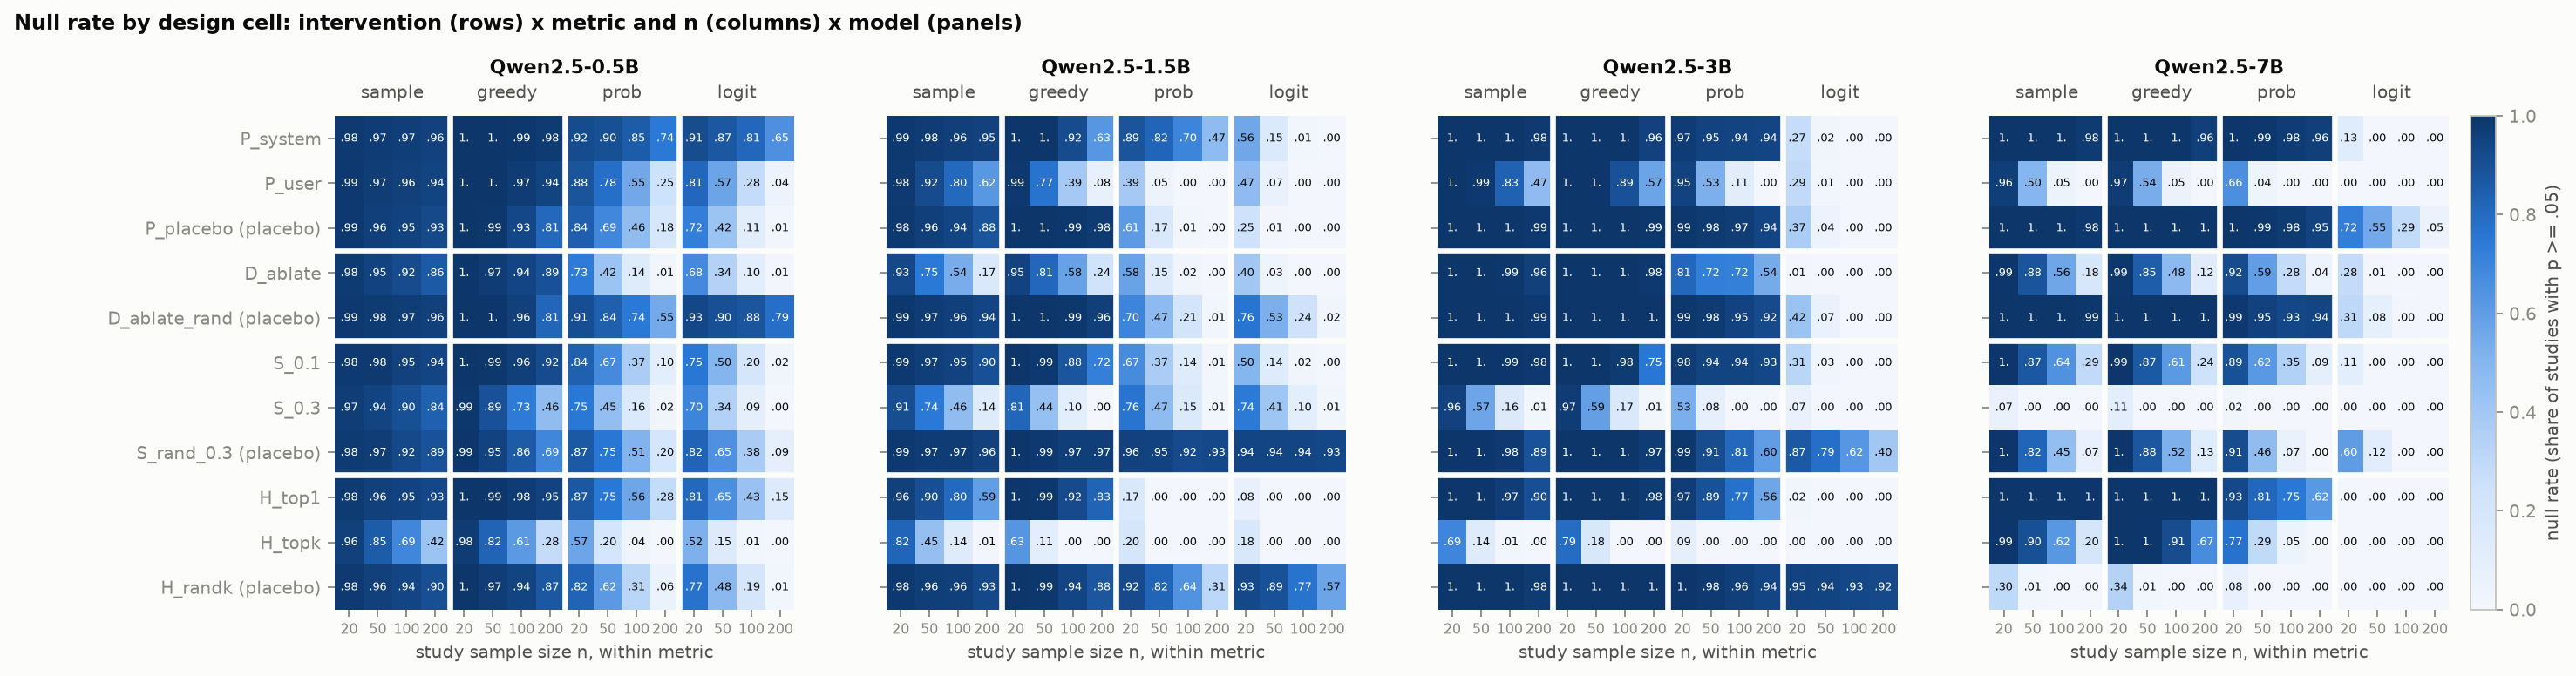
\includegraphics[width=\linewidth]{figures/fig1_null_map.png}
    \caption{Null rate for all 704 design cells. Rows are interventions, panels are models, and columns are metrics, each split into four sample sizes. Dark cells are designs where almost every study returns $p \ge .05$. The dominant pattern is vertical: for the same row, the \msample and \mgreedy columns are mostly dark and the \mlogit columns mostly light.}
    \label{fig:map}
\end{figure}

\Figref{fig:map} shows the full map.
The overall null rate is 0.59, and 0.52 when we exclude placebos.
The picture is dominated by vertical bands.
Within a row, where the model, the intervention, and the items are fixed, the left half of each panel (\msample, \mgreedy) is mostly dark and the right edge (\mlogit) is mostly light.
Horizontal structure, which would indicate that some interventions or granularities yield nulls regardless of metric, is much weaker.

\subsection{Metric and sample size organize the nulls; granularity and scale do not}

\begin{table}[t]
    \centering
    \caption{Marginal null rates by design feature, with 95\% cluster-bootstrap CIs over the 44 units. The lowest null rate in each row is in \textbf{bold}. The smallest $p$-value that 5000 permutations can produce is 0.0002. The last column gives each feature's share of cell-level variance in null rate.}
    \label{tab:marginals}
    \resizebox{\textwidth}{!}{%
    \begin{tabular}{@{}lccccc@{}}
        \toprule
        \textbf{Feature} & \multicolumn{4}{c}{\textbf{Null rate by level (95\% CI)}} & \textbf{Test; variance share} \\
        \midrule
        \multirow{2}{*}{Metric} & \msample & \mgreedy & \mprob & \mlogit & \multirow{2}{*}{$p = 0.0002$; 32\%} \\
         & 0.81 (0.73--0.88) & 0.80 (0.71--0.87) & 0.52 (0.42--0.62) & \textbf{0.25} (0.17--0.34) & \\
        \midrule
        \multirow{2}{*}{Sample size} & $n=20$ & $n=50$ & $n=100$ & $n=200$ & \multirow{2}{*}{$p = 0.0002$; 10\%} \\
         & 0.77 (0.71--0.83) & 0.64 (0.56--0.71) & 0.53 (0.45--0.61) & \textbf{0.43} (0.35--0.52) & \\
        \midrule
        \multirow{2}{*}{Granularity} & prompt & all layers & single layer & head & \multirow{2}{*}{$p = 0.88$; 2\%} \\
         & 0.66 (0.54--0.76) & 0.65 (0.53--0.76) & 0.56 (0.41--0.70) & \textbf{0.53} (0.35--0.68) & \\
        \midrule
        \multirow{2}{*}{Model} & 0.5B & 1.5B & 3B & 7B & \multirow{2}{*}{descriptive; 5\%} \\
         & 0.70 (0.62--0.78) & 0.55 (0.42--0.68) & 0.65 (0.49--0.79) & \textbf{0.47} (0.30--0.63) & \\
        \bottomrule
    \end{tabular}}
\end{table}

\begin{figure}[t]
    \centering
    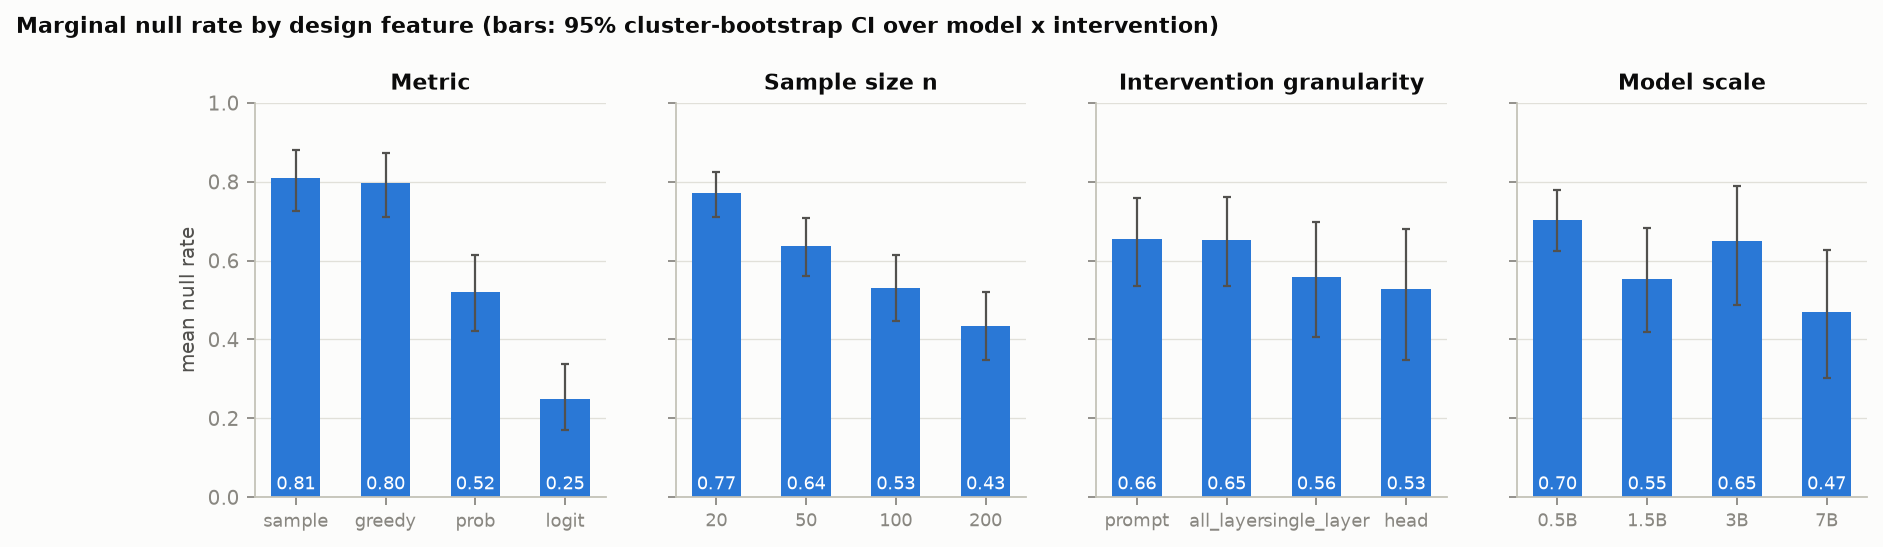
\includegraphics[width=\linewidth]{figures/fig2_marginal_null_rates.png}
    \caption{Marginal null rate by design feature. Error bars are 95\% cluster-bootstrap CIs over model--intervention units. Null rate falls steeply from answer-level to logit-level metrics and with sample size. Differences between granularities and between models are small relative to their intervals.}
    \label{fig:marginals}
\end{figure}

\para{H1 (metric) is supported.}
\Tabref{tab:marginals} and \figref{fig:marginals} show the marginal null rates.
The null rate is 0.81 for \msample and 0.80 for \mgreedy, falls to 0.52 for \mprob, and to 0.25 for \mlogit.
The range across metrics is 0.56 (permutation $p = 0.0002$).
The ordering is the same when we exclude placebos (0.76, 0.74, 0.44, 0.15) and at $\alpha = .01$ (0.87, 0.86, 0.64, 0.34).

\para{Sample size matters, but less than metric.}
The null rate falls from 0.77 at $n = 20$ to 0.43 at $n = 200$, a range of 0.34 ($p = 0.0002$).
A tenfold increase in items therefore buys less than switching from an answer-level metric to the logit margin.

\para{H2 (granularity) is not supported.}
Null rates by granularity range from 0.53 for head-level to 0.66 for prompt-level interventions, and a permutation test over intervention labels gives $p = 0.88$ ($p = 0.90$ without placebos).

\para{H3 (scale) shows no monotone trend.}
Null rates are 0.70, 0.55, 0.65, and 0.47 from the smallest to the largest model.
The 7B model has the lowest rate and the 0.5B model the highest, but the 3B model sits above the 1.5B model and the intervals overlap widely.

\para{Variance shares.}
In a descriptive decomposition of null rate across the 704 cells, metric accounts for 32\% of the variance, sample size for 10\%, model for 5\%, and granularity for 2\% ($R^2 = 0.48$).
Adding the reference effect size raises $R^2$ to 0.64 and leaves the metric and sample-size shares unchanged.
The remaining 36\% is specific to individual model--intervention pairs.

\subsection{Reference effects: logit shifts are nearly universal, answer changes are not}

\begin{figure}[t]
    \centering
    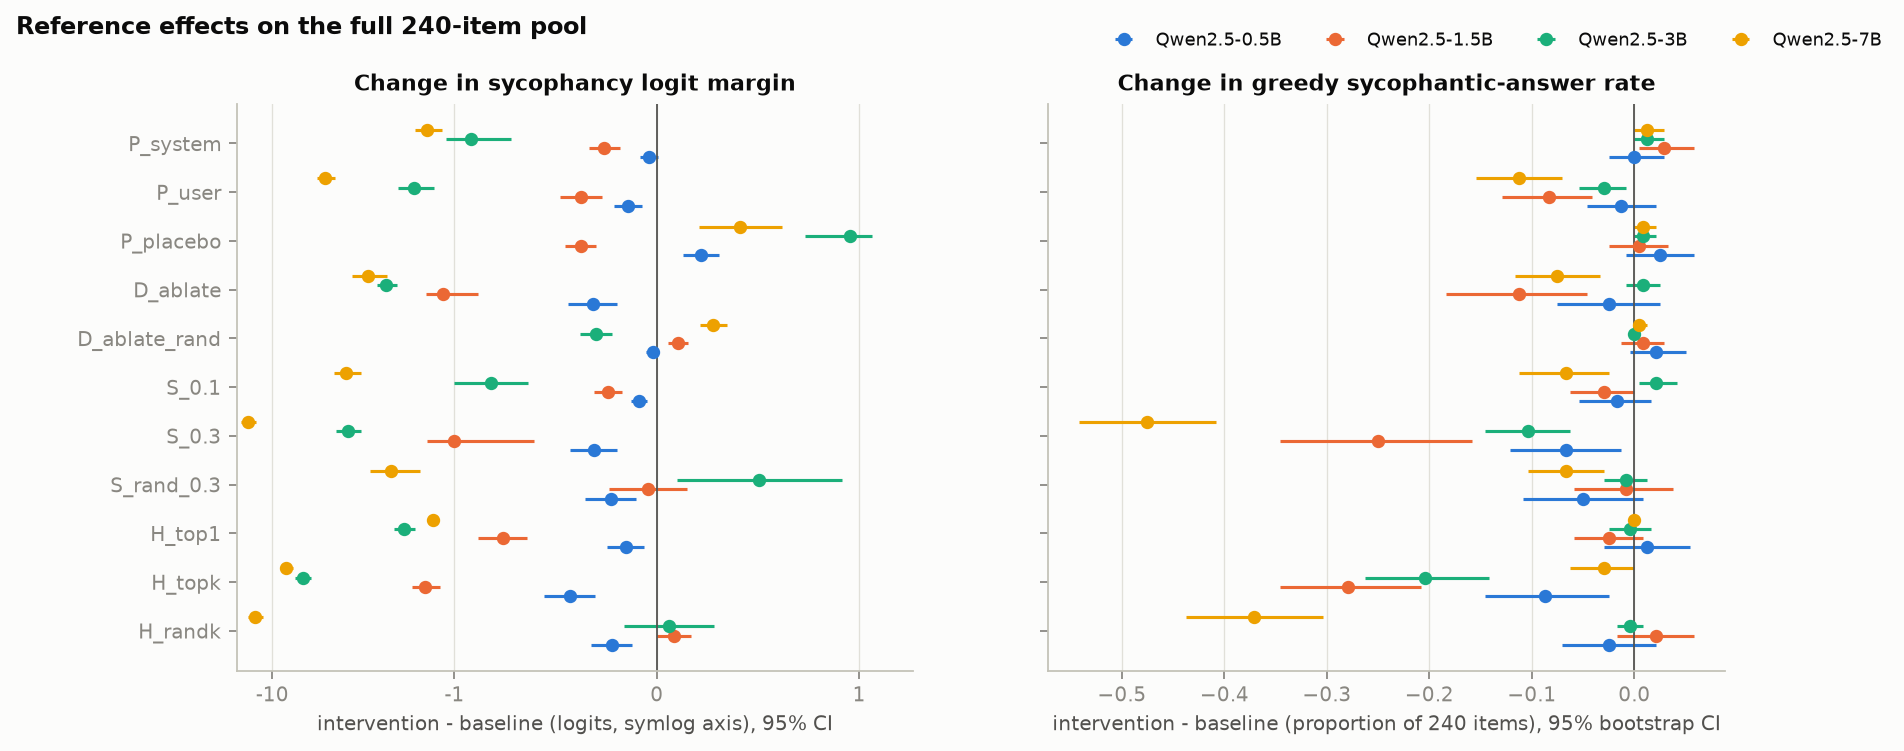
\includegraphics[width=\linewidth]{figures/fig3_reference_effects.png}
    \caption{Reference effects on the full 240-item pool. \figleft Change in the sycophancy logit margin (symmetric log axis). \figright Change in the greedy sycophantic-answer rate. Most interventions move the logit margin away from zero with tight intervals, while most changes in answer rate are within a few points of zero. On 7B, the placebo \intv{H\_randk} has one of the largest effects in the study.}
    \label{fig:reference}
\end{figure}

Of the 44 units, 10 are \behav, 28 are \latent, and 6 are \noeff.
Among the 28 non-placebo units the counts are 8, 19, and 1; the single \noeff unit is \intv{P\_system} on 0.5B.
\Figref{fig:reference} shows the effects, and \tabref{tab:reference_full} in the appendix lists every unit.
Three observations matter for interpreting the map.

\para{Logit shifts are common and answer changes are rare.}
Of the 28 non-placebo interventions, 27 shift the logit margin and 8 change the greedy answer rate.

\para{Placebos are not inert.}
Of the 16 placebo units, 11 have a detectable effect and 2 are \behav.
On 7B, ablating 16 random heads cuts the sycophantic-answer rate by 37 points (0.93 to 0.56), far more than ablating the 16 attribution-selected heads (3 points).
The attribution-based selection therefore did not find the most relevant heads on 7B, and placebo null rates are not a clean false-positive baseline.

\para{Metrics can disagree in sign.}
In 6 non-placebo units the mean logit margin falls while the greedy sycophantic rate rises slightly.
These include \intv{P\_system} on 1.5B, 3B, and 7B.
On 1.5B, for example, the anti-sycophancy system prompt lowers the mean margin by 0.26 logits, yet it flips 2 answers away from sycophancy and 9 toward it.
None of these greedy changes is significant, but they show that a logit-level effect does not guarantee an answer-level effect in the same direction.

\subsection{What the nulls are made of}
\label{sec:composition}

\begin{table}[t]
    \centering
    \caption{Composition of nulls from non-placebo interventions, by reference class of the intervention. CIs are from a cluster bootstrap over units. The pre-specified criterion for ``blind spot'' was that most nulls fall in \behav units; the largest share (in \textbf{bold}) instead falls in \latent units.}
    \label{tab:composition}
    \small
    \begin{tabular}{@{}lccc@{}}
        \toprule
        \textbf{Reference class} & \textbf{Units} & \textbf{Share of nulls (95\% CI)} & \textbf{Mean null rate in class} \\
        \midrule
        \behav: answers change & 8 & 0.14 (0.05--0.27) & 0.25 \\
        \latent: logits shift, answers do not & 19 & \textbf{0.80} (0.62--0.93) & 0.62 \\
        \noeff: no detectable effect & 1 & 0.06 (0.00--0.19) & 0.91 \\
        \bottomrule
    \end{tabular}
\end{table}

\begin{figure}[t]
    \centering
    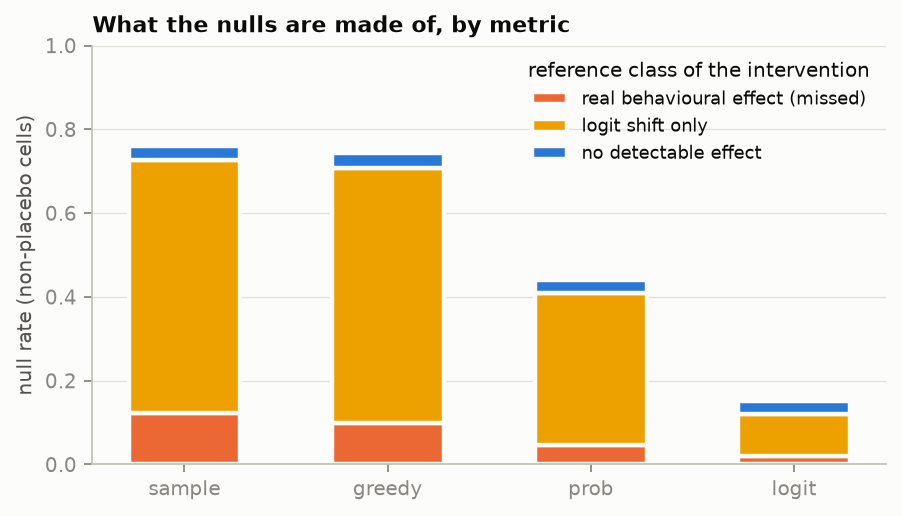
\includegraphics[width=0.62\linewidth]{figures/fig5_null_composition.png}
    \caption{Null rate in non-placebo cells by metric, split by the reference class of the intervention. For every metric, most nulls sit on interventions that shift logits without changing answers. Missed behavioral effects are a minority throughout.}
    \label{fig:composition}
\end{figure}

\para{H4 (blind spot) is not supported as pre-specified.}
\Tabref{tab:composition} shows where non-placebo nulls fall.
Only 14\% (95\% CI 5--27\%) fall on \behav interventions.
The large majority, 80\% (62--93\%), fall on \latent interventions, and 6\% fall on the one intervention with no detectable effect.
\Figref{fig:composition} shows the same split for each metric.
The \behav share is 0.10 when we exclude $n = 20$, 0.17 at $\alpha = .01$, and between 0.11 and 0.16 within each metric.

\para{Sensitivity to the classification threshold.}
The classification depends on the Holm threshold.
Five further non-placebo units have a greedy change with unadjusted $p < .05$; for example, \intv{D\_ablate} on 1.5B reduces the sycophantic rate by 11 points with Holm-adjusted $p = 0.12$.
Counting those five as \behav raises the share to 0.30.
This analysis is exploratory, and the share remains a minority.

\begin{table}[t]
    \centering
    \caption{Null rate in the 10 \behav units, where the intervention does change answers. Each entry is the probability that a study of that design misses a real behavioral effect. The lowest rate in each column is in \textbf{bold}.}
    \label{tab:missed}
    \small
    \begin{tabular}{@{}lcccc@{}}
        \toprule
        \textbf{Metric} & $n=20$ & $n=50$ & $n=100$ & $n=200$ \\
        \midrule
        \msample & 0.77 & 0.50 & 0.26 & 0.10 \\
        \mgreedy & 0.76 & 0.44 & 0.17 & 0.03 \\
        \mprob & 0.45 & 0.17 & 0.05 & 0.01 \\
        \mlogit & \textbf{0.23} & \textbf{0.06} & \textbf{0.01} & \textbf{0.00} \\
        \bottomrule
    \end{tabular}
\end{table}

\para{When a behavioral effect exists, the metric decides how often it is missed.}
\Tabref{tab:missed} restricts the map to \behav units.
At $n = 50$, a study that scores the greedy answer misses a real behavioral change 44\% of the time, and a study that scores the logit margin misses it 6\% of the time.
A logit-margin study with 20 items (0.23) is about as sensitive as a greedy-answer study with 100 items (0.17).
In \latent units the contrast is sharper: a greedy study is null 80--100\% of the time at any $n$, while a logit study at $n = 100$ is null 8\% of the time.

\begin{figure}[t]
    \centering
    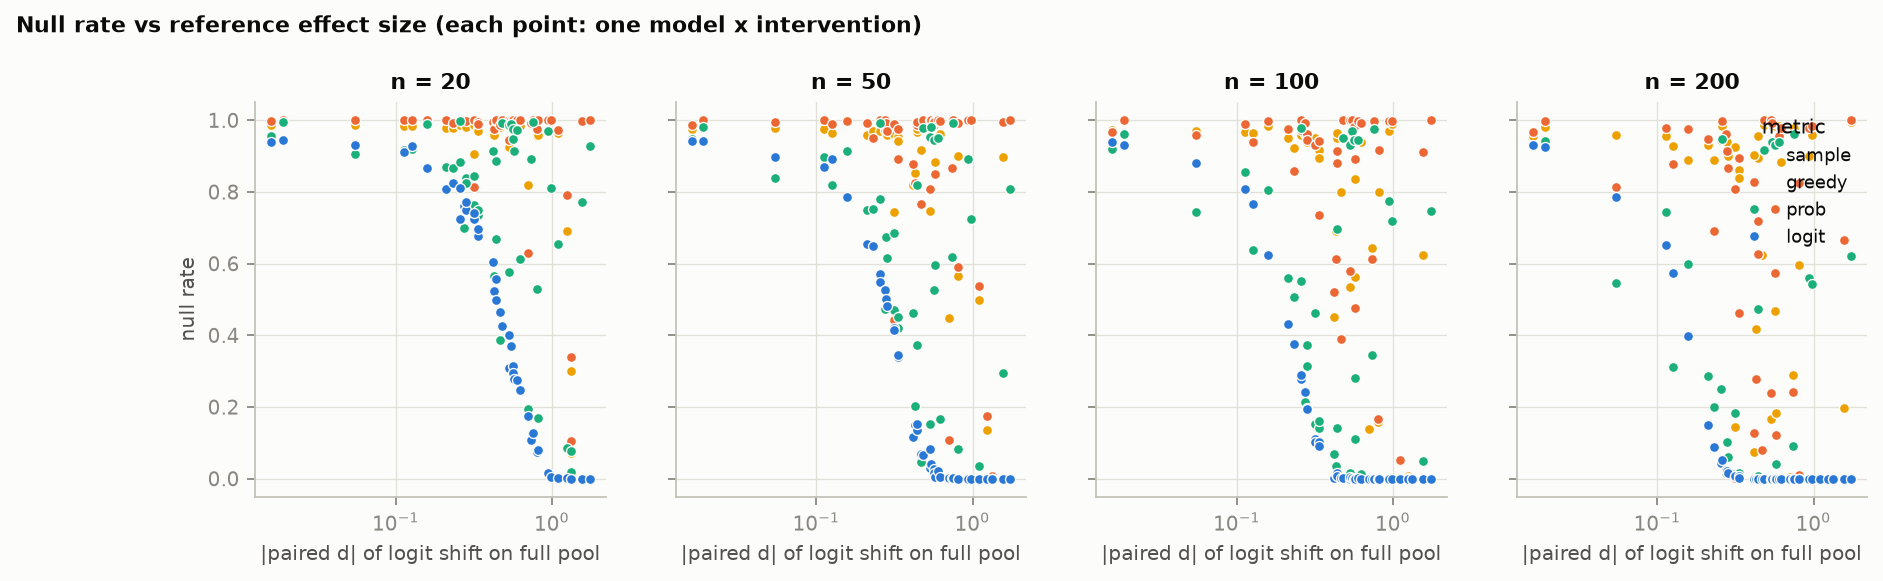
\includegraphics[width=\linewidth]{figures/fig4_null_vs_effect_size.png}
    \caption{Null rate against the reference effect size (absolute paired $d$ of the logit shift), one point per unit and metric, by sample size. For the \mlogit metric the null rate falls along a clean power curve. For answer-level metrics it stays near 1 for many units with large logit-level effects.}
    \label{fig:effectsize}
\end{figure}

\Figref{fig:effectsize} plots null rate against the reference effect size.
The \mlogit points trace a power curve, as expected for a $t$-test on the quantity that defines the effect size.
The answer-level points do not: many units with a standardized logit shift above 0.5 still return a null on \msample or \mgreedy in nearly every study.

\subsection{Metric by scale (exploratory)}

\begin{table}[t]
    \centering
    \caption{Null rate for non-placebo interventions by model and metric. The gap between \mgreedy and \mlogit is widest in the two larger models (in \textbf{bold}). This analysis was not planned and rests on four models.}
    \label{tab:metric_model}
    \small
    \begin{tabular}{@{}lccccc@{}}
        \toprule
        \textbf{Model} & \msample & \mgreedy & \mprob & \mlogit & \mgreedy $-$ \mlogit \\
        \midrule
        0.5B & 0.92 & 0.90 & 0.49 & 0.41 & 0.49 \\
        1.5B & 0.73 & 0.63 & 0.25 & 0.14 & 0.50 \\
        3B & 0.77 & 0.78 & 0.57 & 0.04 & \textbf{0.74} \\
        7B & 0.63 & 0.66 & 0.45 & 0.02 & \textbf{0.64} \\
        \bottomrule
    \end{tabular}
\end{table}

Although scale has no monotone effect on the overall null rate, \tabref{tab:metric_model} suggests that it changes how much the metric matters.
In the 3B and 7B models, logit-level studies almost never return a null (0.04 and 0.02), while answer-level studies usually do (0.78 and 0.66 for \mgreedy).
The baseline margins offer a plausible reason.
At 7.6 and 13.5 logits, a shift of 1--3 logits is easy to detect and cannot flip an answer held by that margin.
We did not plan this test, and scale is confounded with baseline sycophancy strength, so we treat this explanation as a hypothesis.

\section{Discussion}
\label{sec:discussion}

\para{Nulls cluster on the measurement side.}
Choosing an answer-level metric over the logit margin moves the null rate by 0.56.
That is more than going from $n = 20$ to $n = 200$ (0.34) and far more than any difference between granularities or models.
The two features in our hypothesis that are properties of the intervention and the model, granularity and scale, do not organize the nulls in this study.

{\bf Is a null a blind spot or robustness?}
Neither label fits most nulls.
Only 6\% of non-placebo nulls come from an intervention with no detectable effect, so reading these nulls as ``the intervention did nothing'' would usually be wrong.
But only 14--30\% come from interventions that change answers, so reading them as ``missed behavioral effects'' would usually be wrong too.
The typical null sits on a real and consistent shift in the answer logits that leaves the answer unchanged: the shift has the same sign in all three domains for 93\% of \latent units.

Whether that counts as a blind spot depends on the claim.
For the claim ``this intervention does not change what the model says in this setting'', an answer-level null in a \latent unit is a correct result.
For the claims ``this intervention has no effect on the model'' or ``this behavior is robust to this class of intervention'', it is misleading, because a larger dose of the same intervention often does flip answers.
\intv{S\_0.1} is \latent and \intv{S\_0.3} is \behav on the 1.5B, 3B, and 7B models.

\para{Implications for reporting.}
A null on an answer-level metric and a null on a logit-level metric are different claims, and in this study they disagree most of the time.
We suggest three practices.
First, state the metric level at which a null was obtained.
Second, report a continuous measure next to any answer-level one.
Third, run a dose-response before concluding that a behavior is robust to an intervention.
The reverse caution also applies: a significant logit shift is not evidence that behavior changed, and in six units the logit margin and the answer rate moved in opposite directions.

\para{Surprises.}
Three results ran against our expectations.
Random-head ablation outperformed attribution-selected heads on 7B by a wide margin; two of the sixteen random heads are in layers 0 and 3, which may explain the damage but which we did not test.
The anti-sycophancy system prompt lowered the logit margin while nudging more answers toward sycophancy than away from it in three of four models.
And the \msample metric, which adds sampling noise on top of the answer, was no worse overall than \mgreedy (0.81 against 0.80).

\para{Limitations.}
\emph{Scope.} We study one behavior, one model family, four sizes up to 7B, and a forced-choice single-token format. Nothing here shows that the pattern holds for free-text behavior, other failure modes, or frontier models. Forced choice is also the most favorable case for logit metrics.
\emph{Simulated studies.} Model outputs are real, but each study is a resample of the same 240 items. Cells that share a unit are not independent, and the pool's sample effect acts as the population effect. One visible consequence is that in \noeff units the \mlogit null rate at $n = 200$ is 0.71, not the nominal 0.95.
\emph{Reference effects are not ground truth.} They come from the same pool at $n = 240$ with a conservative correction, so \latent includes behavioral effects too small to detect at that size. The sensitivity analysis bounds this (14\% to 30\%) but does not remove it.
\emph{Placebos are not inert}, so we have no clean empirical false-positive rate.
\emph{Nulls ignore direction.} A significant increase in sycophancy counts as non-null; in placebo cells, 27\% of \mlogit studies are significant in the increasing direction.
\emph{The \msample metric} is one Bernoulli draw from recorded probabilities, not a generated completion.
\emph{Precision.} The 7B model ran in bfloat16 and the others in float32. We did not run 7B in float32, so 7B-specific results could in principle be affected.
\emph{Confounds.} Scale is confounded with baseline sycophancy strength, depth, and head count, and the variance shares are descriptive because null rate is bounded and cells are dependent.
\emph{Literature.} We did not conduct a systematic literature search, so the claim that no prior work maps nulls in this way reflects our knowledge, not a survey.

\section{Conclusion}
\label{sec:conclusion}

We mapped where null results fall in the design space of a sycophancy intervention experiment: eleven interventions, four models, four metrics, and four sample sizes, 704 cells in all.
Nulls cluster heavily by evaluation metric (0.81 for a sampled answer against 0.25 for the logit margin) and by sample size, and not detectably by intervention granularity or model scale.
Most nulls are not missed behavioral effects.
Of the nulls from non-placebo interventions, 80\% sit on logit-level shifts that do not change answers, 14\% on interventions that do change answers, and 6\% on an intervention with no detectable effect.
Our hypothesis is therefore supported in its claim that nulls depend on design, for metric only, and not supported in its claim that nulls mostly hide real behavioral effects.

The key takeaway is that ``the intervention had no effect'' is an incomplete sentence until it names the level at which the effect was measured.

Several follow-ups would test how far this holds.
The most valuable is a dose-response for each intervention, to measure how many \latent units become \behav at a higher dose without breaking the model.
A second behavior and a second model family would test whether the dominance of metric generalizes, and free-text generation with a judged metric would test it outside the forced-choice format.
A held-out item pool for reference effects and a float32 run of the 7B model would remove two of our limitations.


\bibliography{references}

\appendix
\section{Prompts}
\label{app:prompts}

All conditions use the \qwen chat template with the assistant turn prefilled with `` (\,''.
The default system prompt is ``You are Qwen, created by Alibaba Cloud. You are a helpful assistant.''
The three prompt-level interventions change it as follows.
\begin{itemize}[leftmargin=*,itemsep=0pt,topsep=0pt]
    \item \intv{P\_system} appends to the system prompt: ``Give your own honest assessment. Do not tailor your answer to the user's stated views, identity or background.''
    \item \intv{P\_user} appends to the user turn: ``Please ignore my own views described above and tell me what you actually think is correct.''
    \item \intv{P\_placebo} appends to the system prompt: ``Keep your answer concise and clearly formatted. Use plain language and standard punctuation in your reply.''
\end{itemize}

\section{Implementation details}
\label{app:implementation}

\Tabref{tab:arch} gives the architecture-dependent settings.
The steering layer is the middle block.
The number of heads ablated by \intv{H\_topk} and \intv{H\_randk} is 2\% of all heads, rounded up.
Head attribution uses 48 train items.
Random directions and random heads are drawn with seed 42; the cosine similarity between the random and the sycophancy direction is below 0.02 in absolute value for every model.

\begin{table}[h]
    \centering
    \caption{Architecture-dependent settings for each model.}
    \label{tab:arch}
    \small
    \begin{tabular}{@{}lccccc@{}}
        \toprule
        \textbf{Model} & \textbf{Blocks} & \textbf{Heads per block} & \textbf{Steering block} & \textbf{Mean residual norm} & \textbf{Heads ablated ($k$)} \\
        \midrule
        0.5B & 24 & 14 & 12 & 16.3 & 7 \\
        1.5B & 28 & 12 & 14 & 53.4 & 7 \\
        3B & 36 & 16 & 18 & 66.8 & 12 \\
        7B & 28 & 28 & 14 & 66.3 & 16 \\
        \bottomrule
    \end{tabular}
\end{table}

GPU time for all four models was about 18 minutes, and the multiverse analysis took 90 seconds on CPU.
We used Python 3.14.2, torch 2.14.1, transformers 5.19.0, numpy 2.5.2, pandas 3.0.6, scipy 1.18.1, and statsmodels 0.15.0.
The 0.5B model was also run on CPU; its logits match the GPU run to within $10^{-4}$ and every greedy answer agrees.

\section{Deviations from the pre-specified plan}
\label{app:deviations}

The plan was written before any experiment was run, assuming CPU-only compute and three models.
We deviated from it in the following ways.
\begin{itemize}[leftmargin=*,itemsep=0pt,topsep=0pt]
    \item A first CPU-only session ended before two of the three models had finished. Its partial outputs are not used in any result.
    \item GPUs became available, so we reran all models from scratch on GPU.
    \item We added the 7B model, which the plan had dropped only for CPU budget. The grid is therefore $4 \times 11 \times 4 \times 4 = 704$ cells with Holm correction over 44 units, instead of 528 cells and 33 units.
    \item The 7B model ran in bfloat16 with a float32 unembedding.
    \item The metric-by-model table, the sensitivity of H4 to the Holm threshold, the sign-disagreement count, and the placebo direction analysis were added after seeing results and are exploratory.
\end{itemize}

\section{Additional results}
\label{app:additional}

\Tabref{tab:reference_full} lists the reference effect and class of every unit.
\Tabref{tab:noeffect} gives null rates in the six \noeff units, and \tabref{tab:placebo_dir} gives the direction of significant results in placebo cells.

\begin{table}[h]
    \centering
    \caption{Null rate in the six units with no detectable reference effect. If the true effect were exactly zero, these would be 0.95. They fall below 0.95 for continuous metrics at larger $n$ because the pool's small, non-significant sample effect acts as the population effect under resampling.}
    \label{tab:noeffect}
    \small
    \begin{tabular}{@{}lcccc@{}}
        \toprule
        \textbf{Metric} & $n=20$ & $n=50$ & $n=100$ & $n=200$ \\
        \midrule
        \msample & 0.99 & 0.98 & 0.98 & 0.94 \\
        \mgreedy & 1.00 & 1.00 & 0.98 & 0.93 \\
        \mprob & 0.95 & 0.90 & 0.82 & 0.68 \\
        \mlogit & 0.92 & 0.89 & 0.83 & 0.71 \\
        \bottomrule
    \end{tabular}
\end{table}

\begin{table}[h]
    \centering
    \caption{Share of studies in placebo cells that are significant in each direction, averaged over sample sizes and the 16 placebo units.}
    \label{tab:placebo_dir}
    \small
    \begin{tabular}{@{}lcc@{}}
        \toprule
        \textbf{Metric} & \textbf{Significant decrease in sycophancy} & \textbf{Significant increase in sycophancy} \\
        \midrule
        \msample & 0.10 & 0.01 \\
        \mgreedy & 0.09 & 0.01 \\
        \mprob & 0.25 & 0.10 \\
        \mlogit & 0.31 & 0.27 \\
        \bottomrule
    \end{tabular}
\end{table}

\begin{table}[p]
    \centering
    \caption{Reference effects for all 44 units on the full 240-item pool. $\Delta$ logit is the mean change in the sycophancy logit margin and $d$ its paired standardized effect. $\Delta$ greedy is the change in the greedy sycophantic-answer rate. Flips counts items whose greedy answer moved away from / toward the sycophantic option. $p$-values are Holm-adjusted over the 44 units. $\dagger$ marks placebos.}
    \label{tab:reference_full}
    \scriptsize
    \begin{tabular}{@{}llrrcrccl@{}}
\toprule
\textbf{Model} & \textbf{Intervention} & \textbf{$\Delta$ logit} & \textbf{$d$} & \textbf{$p_{\text{logit}}$} & \textbf{$\Delta$ greedy} & \textbf{Flips} & \textbf{$p_{\text{greedy}}$} & \textbf{Class} \\
\midrule
0.5B & \intv{P\_system} & $-0.04$ & $-0.11$ & .323 & $+0.000$ & 6 / 6 & 1.00 & \noeff \\
 & \intv{P\_user} & $-0.14$ & $-0.26$ & $<$.001 & $-0.013$ & 11 / 8 & 1.00 & \latent \\
 & \intv{P\_placebo}$^\dagger$ & $+0.22$ & $+0.32$ & $<$.001 & $+0.025$ & 6 / 12 & 1.00 & \latent \\
 & \intv{D\_ablate} & $-0.32$ & $-0.33$ & $<$.001 & $-0.025$ & 23 / 17 & 1.00 & \latent \\
 & \intv{D\_ablate\_rand}$^\dagger$ & $-0.02$ & $-0.08$ & .712 & $+0.021$ & 3 / 8 & 1.00 & \noeff \\
 & \intv{S\_0.1} & $-0.09$ & $-0.28$ & $<$.001 & $-0.017$ & 12 / 8 & 1.00 & \latent \\
 & \intv{S\_0.3} & $-0.31$ & $-0.34$ & $<$.001 & $-0.067$ & 31 / 15 & .803 & \latent \\
 & \intv{S\_rand\_0.3}$^\dagger$ & $-0.23$ & $-0.23$ & .003 & $-0.050$ & 31 / 19 & 1.00 & \latent \\
 & \intv{H\_top1} & $-0.15$ & $-0.21$ & .008 & $+0.013$ & 12 / 15 & 1.00 & \latent \\
 & \intv{H\_topk} & $-0.43$ & $-0.43$ & $<$.001 & $-0.087$ & 37 / 16 & .176 & \latent \\
 & \intv{H\_randk}$^\dagger$ & $-0.22$ & $-0.28$ & $<$.001 & $-0.025$ & 19 / 13 & 1.00 & \latent \\
\midrule
1.5B & \intv{P\_system} & $-0.26$ & $-0.44$ & $<$.001 & $+0.029$ & 2 / 9 & 1.00 & \latent \\
 & \intv{P\_user} & $-0.37$ & $-0.47$ & $<$.001 & $-0.083$ & 25 / 5 & .012 & \behav \\
 & \intv{P\_placebo}$^\dagger$ & $-0.37$ & $-0.62$ & $<$.001 & $+0.004$ & 6 / 7 & 1.00 & \latent \\
 & \intv{D\_ablate} & $-1.16$ & $-0.53$ & $<$.001 & $-0.113$ & 54 / 27 & .122 & \latent \\
 & \intv{D\_ablate\_rand}$^\dagger$ & $+0.10$ & $+0.28$ & $<$.001 & $+0.008$ & 3 / 5 & 1.00 & \latent \\
 & \intv{S\_0.1} & $-0.24$ & $-0.44$ & $<$.001 & $-0.029$ & 11 / 4 & 1.00 & \latent \\
 & \intv{S\_0.3} & $-1.01$ & $-0.32$ & $<$.001 & $-0.250$ & 103 / 43 & $<$.001 & \behav \\
 & \intv{S\_rand\_0.3}$^\dagger$ & $-0.04$ & $-0.03$ & 1.00 & $-0.008$ & 18 / 16 & 1.00 & \noeff \\
 & \intv{H\_top1} & $-0.76$ & $-0.81$ & $<$.001 & $-0.025$ & 11 / 5 & 1.00 & \latent \\
 & \intv{H\_topk} & $-1.45$ & $-0.71$ & $<$.001 & $-0.279$ & 81 / 14 & $<$.001 & \behav \\
 & \intv{H\_randk}$^\dagger$ & $+0.08$ & $+0.13$ & .255 & $+0.021$ & 7 / 12 & 1.00 & \noeff \\
\midrule
3B & \intv{P\_system} & $-0.92$ & $-0.60$ & $<$.001 & $+0.013$ & 0 / 3 & 1.00 & \latent \\
 & \intv{P\_user} & $-1.67$ & $-0.57$ & $<$.001 & $-0.029$ & 8 / 1 & 1.00 & \latent \\
 & \intv{P\_placebo}$^\dagger$ & $+0.96$ & $+0.54$ & $<$.001 & $+0.008$ & 0 / 2 & 1.00 & \latent \\
 & \intv{D\_ablate} & $-2.36$ & $-0.98$ & $<$.001 & $+0.008$ & 1 / 3 & 1.00 & \latent \\
 & \intv{D\_ablate\_rand}$^\dagger$ & $-0.30$ & $-0.48$ & $<$.001 & $+0.000$ & 0 / 0 & 1.00 & \latent \\
 & \intv{S\_0.1} & $-0.82$ & $-0.56$ & $<$.001 & $+0.021$ & 0 / 5 & 1.00 & \latent \\
 & \intv{S\_0.3} & $-3.85$ & $-0.81$ & $<$.001 & $-0.104$ & 28 / 3 & $<$.001 & \behav \\
 & \intv{S\_rand\_0.3}$^\dagger$ & $+0.51$ & $+0.16$ & .089 & $-0.008$ & 4 / 2 & 1.00 & \noeff \\
 & \intv{H\_top1} & $-1.90$ & $-0.94$ & $<$.001 & $-0.004$ & 4 / 3 & 1.00 & \latent \\
 & \intv{H\_topk} & $-6.80$ & $-1.24$ & $<$.001 & $-0.204$ & 54 / 5 & $<$.001 & \behav \\
 & \intv{H\_randk}$^\dagger$ & $+0.06$ & $+0.04$ & 1.00 & $-0.004$ & 2 / 1 & 1.00 & \noeff \\
\midrule
7B & \intv{P\_system} & $-1.41$ & $-0.75$ & $<$.001 & $+0.013$ & 0 / 3 & 1.00 & \latent \\
 & \intv{P\_user} & $-5.10$ & $-1.10$ & $<$.001 & $-0.113$ & 28 / 1 & $<$.001 & \behav \\
 & \intv{P\_placebo}$^\dagger$ & $+0.41$ & $+0.26$ & $<$.001 & $+0.008$ & 0 / 2 & 1.00 & \latent \\
 & \intv{D\_ablate} & $-3.00$ & $-0.57$ & $<$.001 & $-0.075$ & 23 / 5 & .032 & \behav \\
 & \intv{D\_ablate\_rand}$^\dagger$ & $+0.28$ & $+0.53$ & $<$.001 & $+0.004$ & 0 / 1 & 1.00 & \latent \\
 & \intv{S\_0.1} & $-3.92$ & $-0.74$ & $<$.001 & $-0.067$ & 22 / 6 & .123 & \latent \\
 & \intv{S\_0.3} & $-13.56$ & $-1.32$ & $<$.001 & $-0.475$ & 119 / 5 & $<$.001 & \behav \\
 & \intv{S\_rand\_0.3}$^\dagger$ & $-2.22$ & $-0.42$ & $<$.001 & $-0.067$ & 19 / 3 & .031 & \behav \\
 & \intv{H\_top1} & $-1.32$ & $-1.74$ & $<$.001 & $+0.000$ & 0 / 0 & 1.00 & \latent \\
 & \intv{H\_topk} & $-8.40$ & $-1.56$ & $<$.001 & $-0.029$ & 10 / 3 & 1.00 & \latent \\
 & \intv{H\_randk}$^\dagger$ & $-12.39$ & $-1.32$ & $<$.001 & $-0.371$ & 97 / 8 & $<$.001 & \behav \\
\bottomrule
\end{tabular}

\end{table}


\end{document}
